%
% Grizzards printable manual
%
% This needs a lot of work yet.
%
% If you're a human, skip to "\mainmatter" to skip over the preamble.
%
\documentclass[10pt,twocolumn,openany,article]{memoir}

\setstocksize{9in}{6in}
\settrimmedsize{\stockheight}{\dimexpr 6in-15mm}{*}

\setlrmarginsandblock{.5in}{1in}{*}
\setulmarginsandblock{.75in}{1in}{*}
\setheadfoot{.5in}{.5in}
\checkandfixthelayout


%% TV Standard

\ifdefined\TVNTSC
\newcommand\TV{NTSC}
\newcommand\REGION{The Americas, Japan, and Korea}
\else
\ifdefined\TVPAL
\newcommand\TV{PAL}
\newcommand\REGION{UK and Western Europe (except France)}
\else
\ifdefined\TVSECAM
\newcommand\TV{SECAM}
\newcommand\REGION{France, Eastern Europe, and Africa}
\else
\error{Must define a TV standard}
\fi
\fi
\fi


\usepackage[utf8]{inputenc}
\usepackage{babel}
\usepackage{stfloats}
\usepackage{microtype}
\usepackage{graphicx}
\usepackage{pdfpages}
\tolerance=1
\emergencystretch=\maxdimen
%\usepackage{tgtermes}
\usepackage{hyperref}
\usepackage{xcolor}
\hypersetup{
    colorlinks,
    linkcolor={red!50!black},
    citecolor={blue!50!black},
    urlcolor={blue!80!black},
    pdftitle={Grizzards \ifdefined\DEMO{ Demo }\fi Manual for \TV},
    pdfsubject={Grizzards videogame for the Atari 2600},
    pdfauthor={Bruce-Robert Pocock}%,
%    pdfkeywords={Your PDF keywords}
  }
\usepackage{caption}
\captionsetup{labelformat=empty}

\usepackage{tikz}

\newcommand\encircle[1]{%
  \tikz[baseline=(X.base)] 
  \node (X) [draw, shape=circle, inner sep=0] {\strut #1};}

\usepackage{lettrine}
\usepackage[protrusion=true,expansion=true]{microtype}
\fontfamily{pnc}
\chapterstyle{komalike}

\checkandfixthelayout

\title{Grizzards \ifdefined\NOSAVE No-Save \fi\ifdefined\DEMO Demo \fi Player's Guide}
\author{Bruce-Robert Pocock}

%
%
%
%%% BEGIN DOCUMENT
%
%
%

\begin{document}
\frontmatter
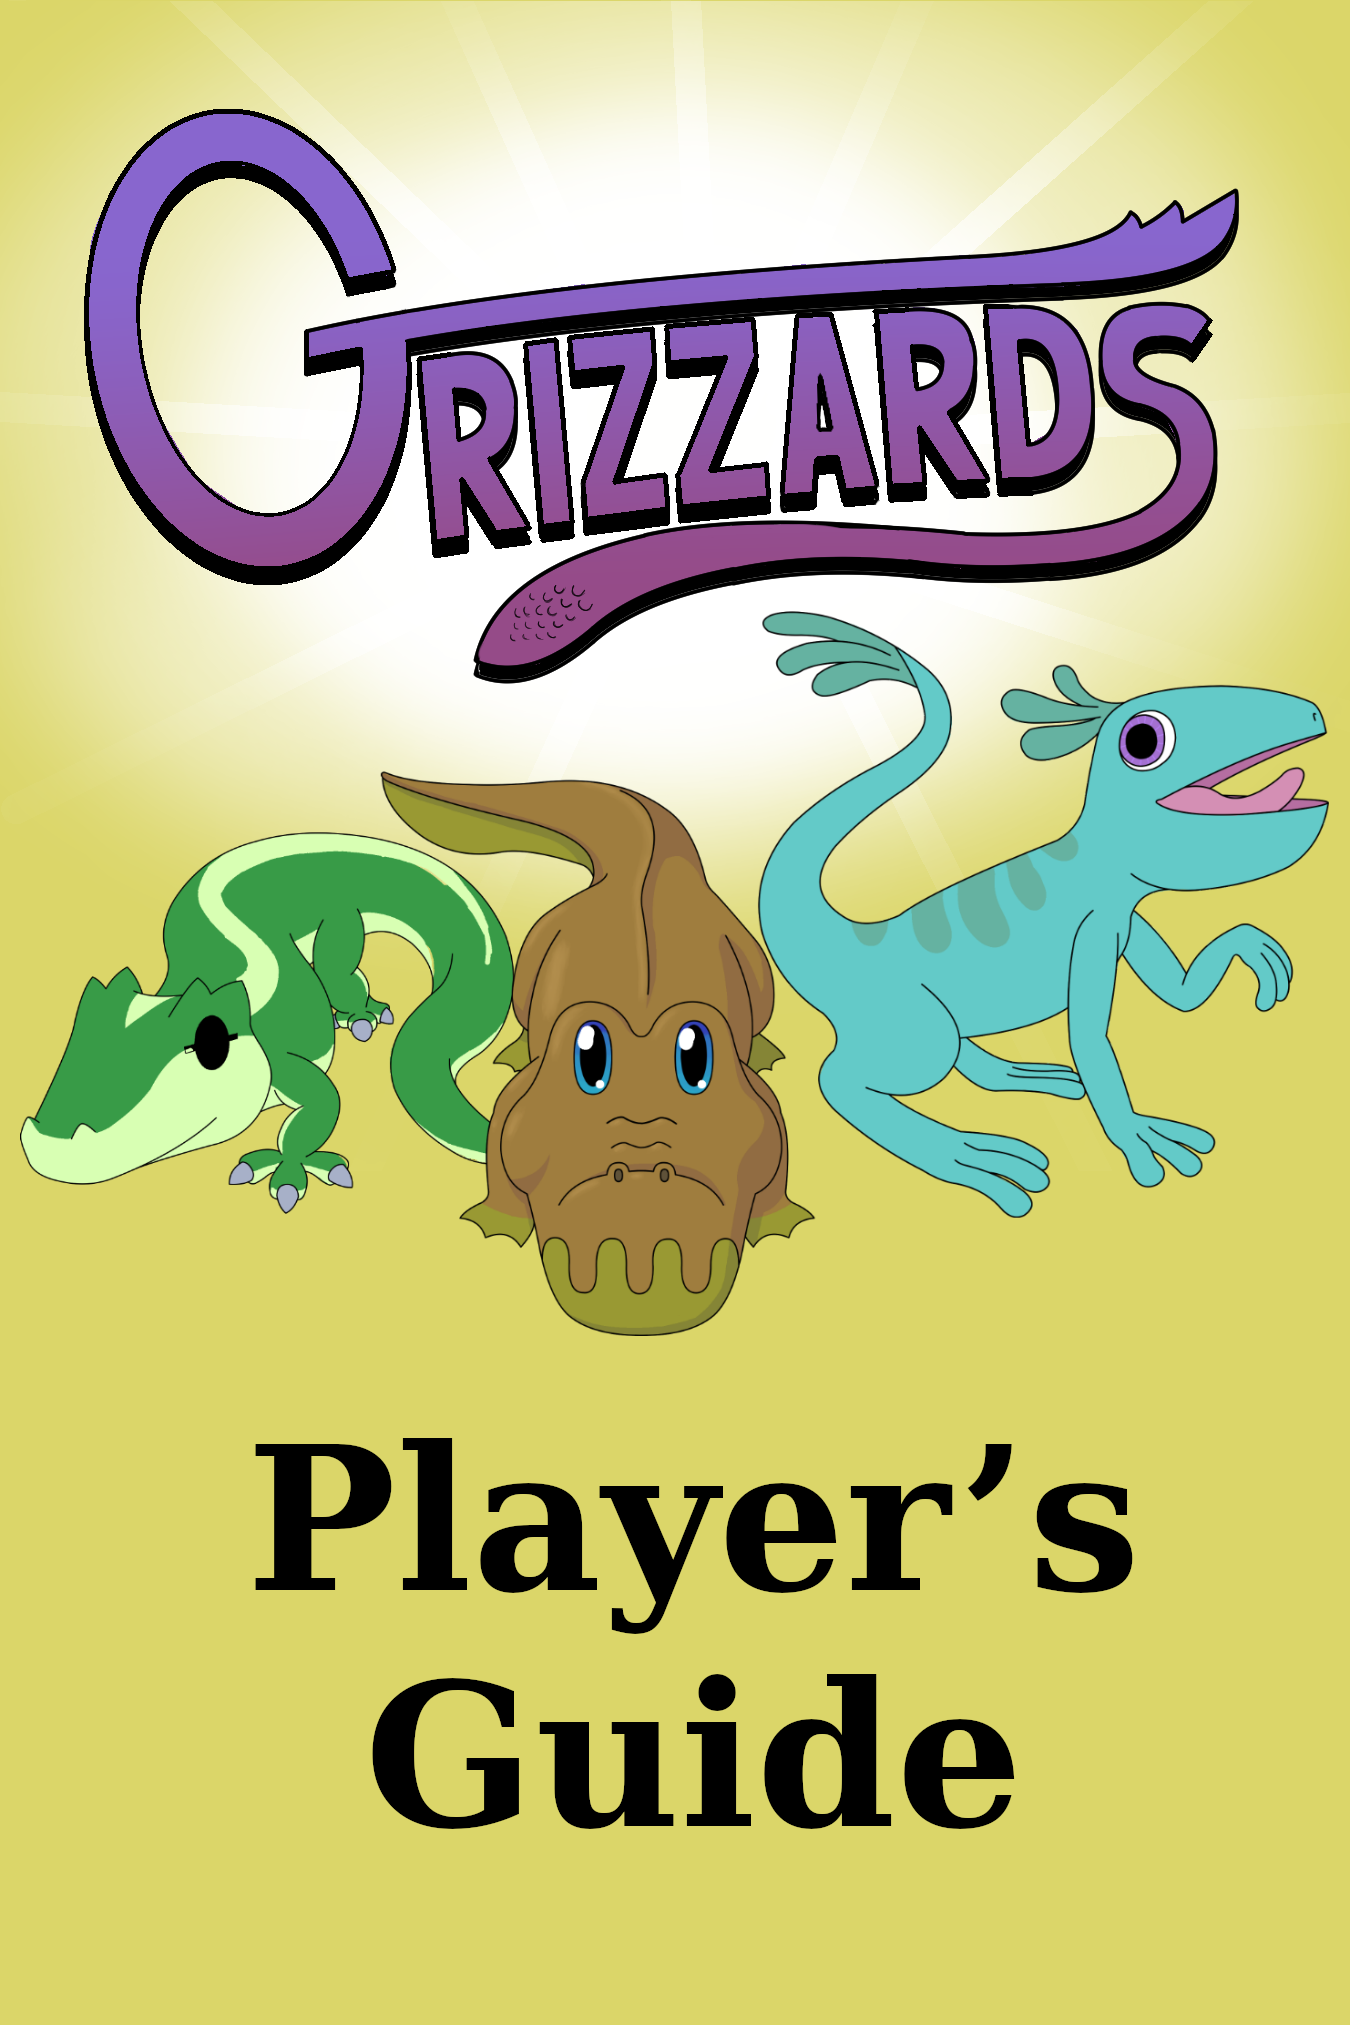
\includepdf[height=9in,width=6in,fitpaper=true]{../Manual/Cover.png}

\thispagestyle{empty}


\twocolumn[

\chapter*{Introduction}\label{Introduction}

The  land of  Syrex  is  a dangerous  place.  Fierce  monsters roam  the
countryside. But luckily for you, you're a Grizzard handler!

Train your Grizzard to  use a variety of moves to  take on the monsters.
Discover new kinds  of Grizzards with new capabilities.  Can you conquer
all the monsters of Syrex?

\bigskip

In the  \textit{Grizzards} videogame, you'll  roam the land  looking for
monsters. Monsters may  surprise you as you travel, or  you may see them
coming. When faced  with terrifying beasts, you'll  direct your Grizzard
to use its moves to defend you and attack the monsters.

\vspace{1in}\vfill

This    is    the     \textit{Grizzards}    \ifdefined\NOSAVE    No-Save
\fi\ifdefined\DEMO Demo \fi\ifdefined\ATARIAGESAVE Official \else Public
Release \fi Player's Guide

Copyright \copyright{} 2021-2022, Bruce-Robert Pocock

\bigskip

This  version is  for systems  in \REGION{}  using the  \TV{} television
standard. For Atari  Video Computer System CX-2600  (or Sears Tele-Games
Video  Arcade  or  Atari 7800  ProSystem)  \ifdefined\ATARIAGESAVE  with
optional AtariVox device. \else \ifdefined\NOSAVE without \else with \fi
AtariVox (or MemCard, or SaveKey) device. \fi

\bigskip

This videogame software was not created, published, or licensed by Atari
or its successors.

\ifdefined\DEMO
\bigskip

This manual  describes a \ifdefined\NOSAVE  No-Save \fi DEMO  version of
the game. The full version may be different.

\fi

Published by AtariAge.

\ifdefined\ATARIAGESAVE\else  If you  enjoy playing  \textif{Grizzards},
you  may  be  interested  in  purchasing a  retail  copy  with  built-in
save-game    memory    from    AtariAge.    Coming    in    2022.    \fi
\href{https://atariage.com/}{https://atariage.com/}

\bigskip

You are hereby granted permission  to make use of the \textit{Grizzards}
videogame software for \emph{non-commercial personal use}.

Redistribution not for profit is allowed, but sales of this software
requires a license.

]

\let\cleardoublepage\clearpage

\mainmatter

\tableofcontents

\twocolumn[ \chapter{Setting Up}\label{Setting Up} ]

To play \textit{Grizzards}, you will need:

\begin{itemize}
\item An Atari  console: the Atari Video Computer  System CX-2600, Sears
  Tele-Games  Video Arcade,  Atari  2600jr game  system,  or Atari  7800
  ProSystem
\item A TV or video display
\item A joystick controller
  \ifdefined\ATARIAGESAVE
  \item Optional: an AtariVox device with speakers or headphones
  \else
  \ifdefined\NOSAVE\else
\item A  memory device: an  AtariVox device with (optional)  speakers or
  headphones, or a MemCard or SaveKey device.
  \fi\fi
\item The \textit{Grizzards} game cartridge \ifdefined\ATARIAGESAVE\else
  or a multi-cart with the \textit{Grizzards} data on it. \fi
\end{itemize}

\ifdefined\NOSAVE\else
\begin{figure*}[b]
  \begin{center}
    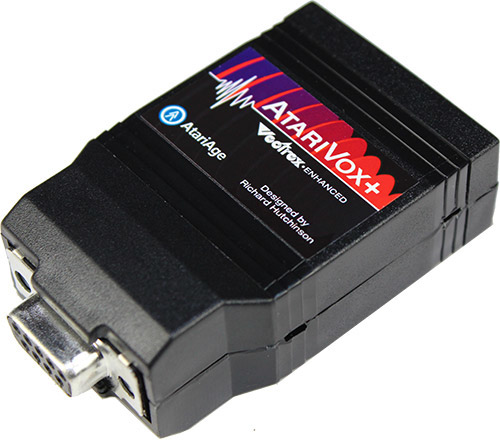
\includegraphics[width=\columnwidth]{../Manual/AtariVox.jpeg}
    \ifdefined\ATARIAGESAVE
    \includegraphics[width=\columnwidth]{../Manual/Atari-2600-Wood-4Sw-Set.png}
    \else
    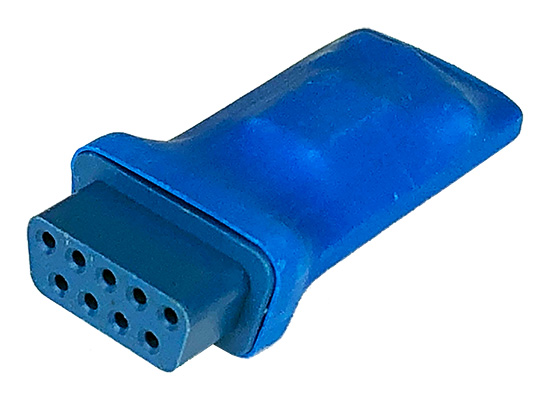
\includegraphics[width=\columnwidth]{../Manual/SaveKey.jpeg}
    \fi
  \end{center}
\end{figure*}
\fi

Set up your console with your TV or video display. Connect a joystick to
the \emph{left} controller port\ifdefined\ATARIAGESAVE, and (optionally)
your   AtariVox   device   to    the   \emph{right}   controller   port.
\else\ifdefined\NOSAVE.\else{},   and   the   memory   device   to   the
\emph{right} controller port.

Note that  the retail  cartridge available later  in 2022  from AtariAge
will \emph{not}  require a  memory device  because the  special AtariAge
cartridge contains its own save-game memory within it.

To purchase \textit{Grizzards}, SaveKey,  AtariVox+, or many other Atari
games,                                                             visit
\href{https://atariage.com/store/}{https://AtariAge.com/store/}

\fi\fi

Finally, insert  the \textit{Grizzards}  game cartridge (with  the label
facing  up)  into  the  cartridge  slot,  and  turn  the  \textbf{Power}
\textbf{on}.

\ifdefined\ATARIAGESAVE\else
\begin{figure}[h]
  \begin{center}
    \includegraphics[width=\columnwidth]{../Manual/Atari-2600-Wood-4Sw-Set.png}
  \end{center}
\end{figure}
\fi

\section{Using a Gamepad}

A  SEGA  \ifdefined\TVNTSC{Genesis/}\fi{}MegaDrive   gamepad  (or  other
compatible controller) may also be  used. Use the \encircle{B} button as
the \textbf{Fire} button. Use the  \encircle{C} button as an alternative
way  to   press  the   \textbf{Game  Select}   switch  to   access  your
Grizzard's statistics.

A ``Joy2b+'' game pad such as those from RetroGameBoyz can also be used.
Button   \encircle{I}   will   work   as   the   \textbf{Fire}   button.
Button \encircle{II} will work as the \textbf{Game Select} switch.

An    Atari     7800    controller     will    \emph{not}     work    as
a two-button controller.

Your gamepad  \emph{must} be  plugged in \emph{before}  you turn  on the
power,    or    the   extra    button    function    will   not    work.
\ifdefined\ATARIAGESAVE\else If  using a \ifdefined\DEMO Harmony  or \fi
Harmony  Encore cartridge,  hold down  the \encircle{B}  or \encircle{I}
button when you power  on your console, or the gamepad  will not work on
the Harmony menu. \fi

\vfill

\columnbreak
\chapter{How To Play}

\section{Console Controls}

\ifdefined\TVSECAM

\subsection{Color/B\&W Switch}

On  a  SECAM Atari  2600  (or  similar console)  the  \textbf{Color/B\&W
  Switch} controls the visuals from  your console. In the \textbf{Color}
position,  your  display will  appear  in  color; in  the  \textbf{B\&W}
position, the game will appear in shades of gray.

\else

\subsection{Color/B\&W Switch (Pause)}

On an Atari 2600  (or similar console) you can pause  the game using the
\textbf{Color/B\&W Switch}. Push the \textbf{Color/B\&W} switch into the
\textbf{Color} position to play, or  the \textbf{B\&W} position to pause
the game.

On the  Atari 7800, press  the \textbf{Pause}  button once to  pause the
game, and  again to  resume playing.  \ifdefined\ATARIAGESAVE\else Note:
this may not work with certain multi-carts, e.g. the UnoCart. \fi

\fi

\subsection{Game Select}

When  viewing the  Title Screen,  you can  use the  \textbf{Game Select}
switch to
\ifdefined\NOSAVE
begin your game or start over
\else
choose the Slot you wish to use to save your progress.
\fi

While you  are playing the  game, you  can use the  \textbf{Game Select}
switch to view your Grizzard's  statistics from the Map screen, Combat
screen, or a Grizzard Depot.

\subsection{Game Reset}

When  viewing the  Select  Slot screen,  press  the \textbf{Game  Reset}
switch to begin playing the game.

While you are playing the game,  press the \textbf{Game Reset} switch to
\emph{immediately} abandon your progress and return to the Title Screen.
You will  lose some  of your  progress since the  last time  you visited
a Grizzard Depot.

\subsection{Difficulty Switches}

\ifdefined\NOSAVE\else

You  cannot erase  a  game  in progress  (or  un-erase  it) unless  both
Difficulty  Switches are  in the  ``A'' (Advanced  or Expert)  position.
To protect your game from being erased, set either one of the Difficulty
Switches to the ``B'' (Beginner or Novice) position.

On the Atari  7800, note that the Difficulty Switches  (located near the
controller  ports) are  in the  ``A'' position  when they  are moved  to
the right.

\fi

\subsubsection*{Expert Mode}

The Left Difficulty Switch adjusts the  difficulty of the game. When the
Left Difficulty  Switch is in  the ``A'' (Advanced or  Expert) position,
monsters will do more damage in  their attacks. When the Left Difficulty
Switch is in  the ``B'' (Beginner or Novice) position,  monsters will do
their normal  amount of  damage. You  will also  earn double  points for
defeating monsters while in the ``A'' position.

\ifdefined\TVSECAM

\subsubsection*{Game Pause}

The Right Difficulty Switch  can be used to pause game  play. When in the
``A'' (Advanced or Expert) position, your  game will be paused until you
toggle the switch to the ``B'' (Beginner or Novice) position.

\fi

\section{Start a Game}

\begin{center}
  \includegraphics[width=\columnwidth]{../Manual/TitleAquax\TV.png}
\end{center}

Once your  console is set  up and everything  is connected, turn  on the
\textbf{Power} switch. You'll  see the title screen appear.  If you have
an AtariVox device, you'll also hear the title spoken.

Press the \textbf{Game Select} switch or \textbf{Fire} button to move to
the
\ifdefined\NOSAVE
Begin/Resume screen.

Press the  joystick left or  right to choose whether  to \texttt{RESUME}
your current game  in progress or \texttt{BEGIN} a new  game, then press
\textbf{Game Reset} or the \textbf{Fire} button.

\else
Select Slot screen.

\begin{center}
  \includegraphics[width=\columnwidth]{../Manual/SelectSlot\TV.png}
\end{center}

Press  the \textbf{Game  Select} switch  or move  the joystick  left and
right             to             choose             a             memory
slot\ifdefined\ATARIAGESAVE\else\footnote{Technical   Note:   The   Slot
  number chosen  here is relative to  the three save game  slots used by
  the  \textit{Grizzards} game  program.  Each save  game slot  actually
  occupies 4 blocks on your memory  device.}\fi for your game. There are
\ifdefined\ATARIAGESAVE  eight \else  three \fi  memory slots  possible.
Press  \textbf{Game Select}  or the  joystick left  and right  to rotate
through them. If someone has already begun to play \textit{Grizzards} in
a certain  slot, your  screen will  show ``\texttt{RESUME},''  and their
name  will   appear  as   well.  If   a  slot   is  empty,   you'll  see
``\texttt{BEGIN}'' instead.

If someone has already \emph{won} the  game once, their name will appear
in bright yellow. See New Game Plus, page~\pageref{sec:NewGamePlus}.

\ifdefined\DEMO

\skip

This demo saves your progress in  the ``scratchpad'' area of your memory
device. It's possible that other  games might overwrite and destroy your
saved progress.  This is  just because  it's a demo,  and does  not have
a private area reserved for it.

\skip

\fi

When you have selected the slot you want to begin (or resume), press the
\textbf{Game Reset} switch or \textbf{Fire} button.

\fi

\ifdefined\NOSAVE\else

When you  first choose  to begin a  new game, you  can enter  your name.
Press  forward to  select  the  next letter;  pull  back  to select  the
previous letter.  Press left and right  to move to the  next or previous
position. You  can have up  to six characters  for your name.  After six
characters, the  cursor will turn  pink. Press the  \textbf{Fire} button
to proceed.

\begin{center}
  \includegraphics[width=\columnwidth]{../Manual/NameEntry\TV.png}
\end{center}

\ifdefined\DEMO

In this demo,  you'll always begin with Aquax as  your companion. In the
full game, you can choose from one of three starting Grizzard companions.

\else

Next,  you'll  get to  pick  your  starting  Grizzard. There  are  three
Grizzards  from which  to  choose:  Dirtex, Aquax,  or  Airex. Refer  to
Chapter~\ref{ch:Grizzards}   on  page~\pageref{ch:Grizzards}   for  more
information about each of them.

\begin{center}
  \includegraphics[width=\columnwidth]{../Manual/GrizzardChooser\TV.png}
\end{center}

Press left  and right  to choose  a Grizzard  companion, then  press the
\textbf{Fire} button.

You'll have one  last chance to make sure that  you've entered your name
correctly and chosen the Grizzard  companion you prefer. Push forward on
the joystick to select \texttt{CHANGE}  and edit your name and companion
choice, or  pull back  to choose to  \texttt{BEGIN} your  adventure now.
Press the \textbf{Fire} button.

\begin{center}
  \includegraphics[width=\columnwidth]{../Manual/ConfirmNewGame\TV.png}
\end{center}

\fi
\fi
\ifdefined\NOSAVE

In this no-save demo, you can only  play with one Grizzard at a time ---
starting with Aquax. The demo using  a memory device allows you to catch
other Grizzards. In the full game,  you can choose one of three starting
Grizzard companions.

\fi

\section{Exploring Syrex}

You'll begin in the ruins of  Treble Village after the monsters invaded.
You know that to  the east is the extremely dangerous  Fire Bog, so your
best  bet   is  to  head   west  (left)  and   see  if  there   are  any
other survivors.

Refer to the  map (back cover of  this manual) for some  ideas about the
geography of  Syrex. Other  characters in  the game  will also  give you
advice about places you can go and things you can do.

The Map screen shows your current score  at the top. In the map display,
you'll see the  current area in which you are  traveling. Guide yourself
using the joystick.

You can check your inventory of potions,  and choose to give one to your
current  Grizzard  companion  by   pressing  the  \textbf{Fire}  button.
\ifdefined\DEMO However, there are no potions in this demo. \fi

\begin{center}
  \includegraphics[width=\columnwidth]{../Manual/Map\TV.png}
\end{center}

As you  travel, you may  encounter people  and things; to  interact with
them, simply walk into them.

\lettrine[image=true,                lines=5,               findent=3pt,
nindent=3pt]{../Manual/Monster\TV.png}{A   monster}  (or   a  group   of
monsters) may  sneak up on you  and attack! Other times  you'll see them
waiting for you and can avoid battle  --- or walk up to them when you're
ready to  face them. Particularly  giant monsters look different  on the
map; you'll discover them in your travels.

\lettrine[image=true,                lines=5,               findent=3pt,
nindent=3pt]{../Manual/Depot\TV.png}{A} Grizzard Depot  is a safe space.
Your  Grizzards will  be  healed\ifdefined\NOSAVE{}.{}\else{}, and  your
progress will  be saved \ifdefined\ATARIAGESAVE to  your game cartridge.
\else to your  memory device. \fi You can also  switch which Grizzard is
your  current  companion.  \fi See  page~\pageref{sec:GrizzardDepot}  to
learn more about Grizzard Depots.

\ifdefined\NOSAVE

\lettrine[image=true,                lines=5,               findent=3pt,
nindent=3pt]{../Manual/WildGrizzard\TV.png}{Wild  Grizzards}   roam  the
land sometimes. In this no-save demo, you will have one Grizzard companion at a time,
beginning with  Aquax.

\else

\lettrine[image=true,                lines=5,               findent=3pt,
nindent=3pt]{../Manual/WildGrizzard\TV.png}{Wild  Grizzards}   roam  the
land  sometimes.   You  can   catch  them   when  you   encounter  them.
At  a Grizzard  Depot,  you'll have  the option  to  swap your  Grizzard
companion  between  those you  have  caught,  with  up to  30  different
Grizzards saved  in your  \ifdefined\ATARIAGESAVE game  cartridge. \else
memory device. \fi Each Grizzard you catch will have its own moves and
skill ratings. 

\fi

\lettrine[image=true,                lines=5,               findent=3pt,
nindent=3pt]{../Manual/Door\TV.png}{Doors} lead  you to other  places in
the world.

\vspace{16pt}

\lettrine[image=true,                lines=5,               findent=3pt,
nindent=3pt]{../Manual/Signpost\TV.png}{Signposts} can provide necessary
information to  help you progress. You  might also want to  refer to the
map on the last page of this manual.


\lettrine[image=true,                lines=5,               findent=3pt,
nindent=3pt]{../Manual/Person\TV.png}{Other  people} will  converse with
you and can help  you out. Make sure you talk to  everyone you meet, and
keep in mind  that some people will respond to  you differently based on
what has come before.



\ifdefined\NOSAVE\else

\section{Saving Your Progress}

The game  is automatically  saved whenever you  visit a  Grizzard Depot.
Some progress is  also saved when you travel  between certain locations,
catch a wild Grizzard, or when one Grizzard changes into another.

\ifdefined\ATARIAGESAVE\else

You should leave your memory device connected at all times while playing
the game.

\fi \fi

\section{Grizzard Depots}\label{sec:GrizzardDepot}

To \ifdefined\NOSAVE\else  swap which  Grizzard you're using,  or to  \fi heal
your current Grizzard companion, you'll need to find a Grizzard Depot.

\begin{figure*}[hb]
  \begin{center}
    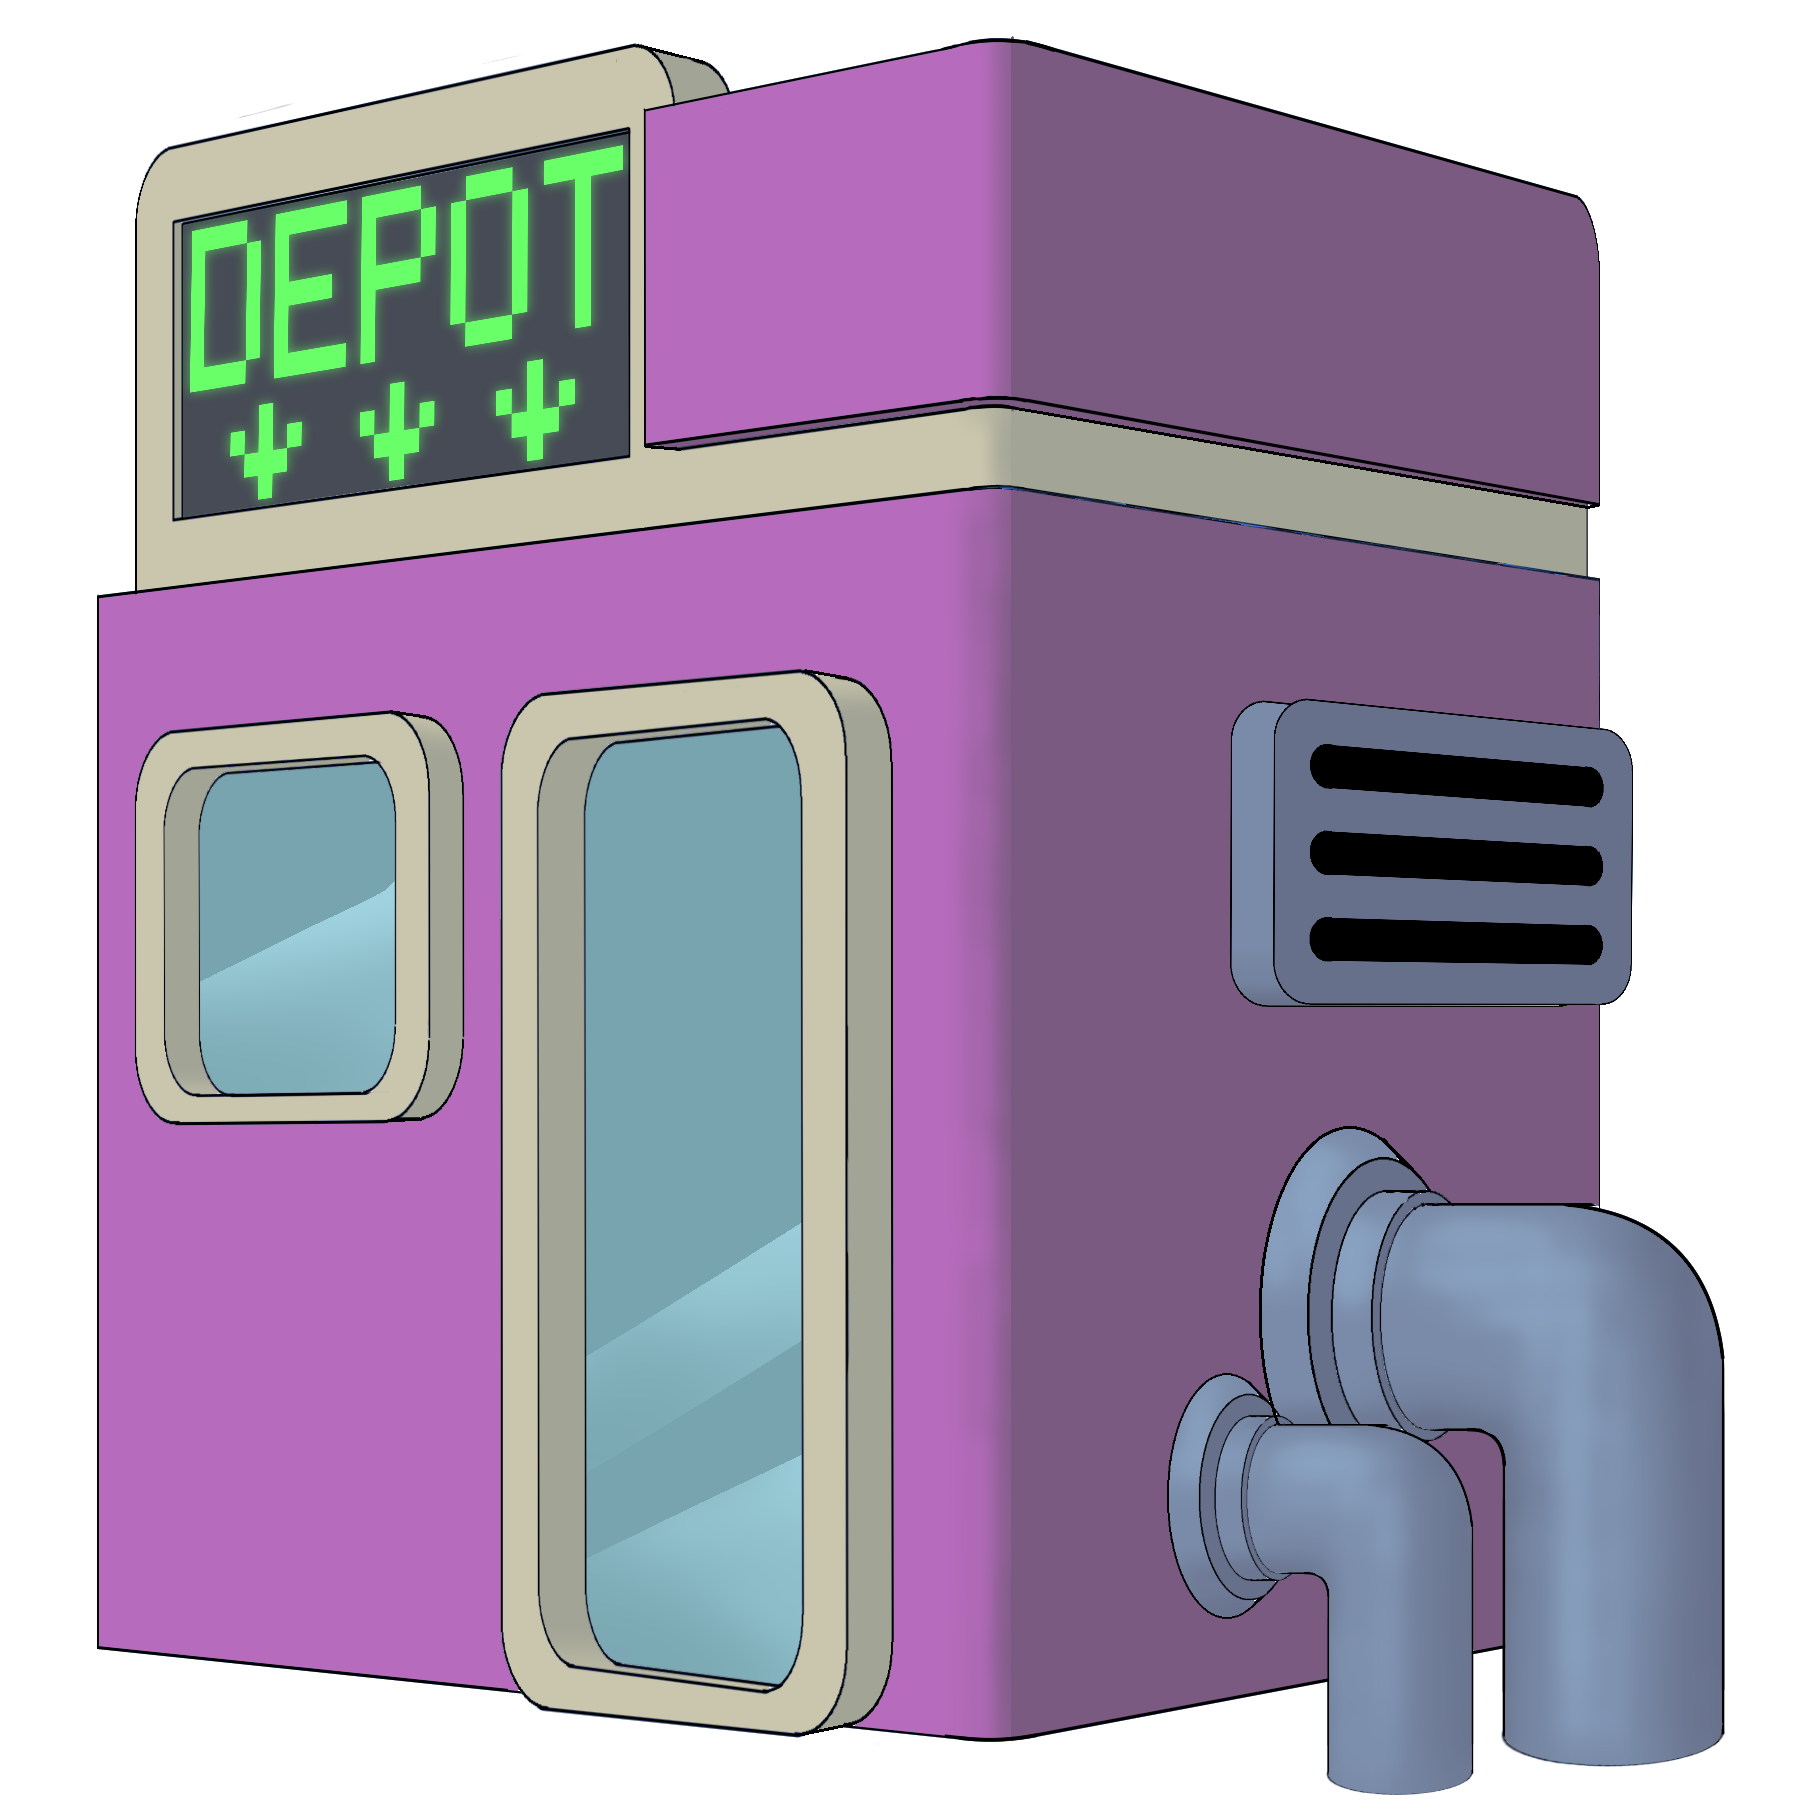
\includegraphics[width=2\columnwidth]{../Manual/GrizzardDepot.png}
  \end{center}
\end{figure*}

\begin{center}
  \includegraphics[width=\columnwidth]{../Manual/DepotScreenshot\TV.png}
\end{center}

Touch the Grizzard Depot on the map screen to enter it.

\ifdefined\NOSAVE\else Your progress will \emph{immediately} be saved to
your \ifdefined\ATARIAGESAVE  game cartridge.  \else memory  device. \fi
\fi

At  a Grizzard  Depot  your  Grizzard companion  will  be fully  healed.
\ifdefined\NOSAVE\else  Press the  joystick forward  and back  to choose
a different Grizzard to travel with you. \fi

To  view  your Grizzard's  statistics,  press  the \textbf{Game  Select}
switch or move  the joystick left or right. When  you're ready to return
to your adventure, press the \textbf{Fire} button.

\section{Conversations}

When you encounter  a person, they'll usually speak to  you. If you have
an AtariVox  connected, you'll hear  what they have  to say out  loud as
well.   After  you've   read  what   they   have  to   say,  press   the
\textbf{Fire} button.

\begin{center}
  \includegraphics[width=\columnwidth]{../Manual/Text\TV.png}
\end{center}

Some people will want to know what you have to say, in return. If that's
the case, you'll be given a choice of two possible answers to give them.
Press forward or back on the joystick to select a response.

\begin{center}
  \includegraphics[width=\columnwidth]{../Manual/Inquire\TV.png}
\end{center}

If  you  want to  review  what  the person  was  asking,  you can  press
left on  the joystick to  ask them to repeat  themself instead.

When you've made your selection, press \textbf{Fire} to continue.

\section{Battling Monsters}

Monsters plague the world of Syrex. If you're caught by monsters without
a  Grizzard companion,  they're sure  to  eat you  alive! Your  Grizzard
companion will defend you.

\begin{figure*}[ht]
  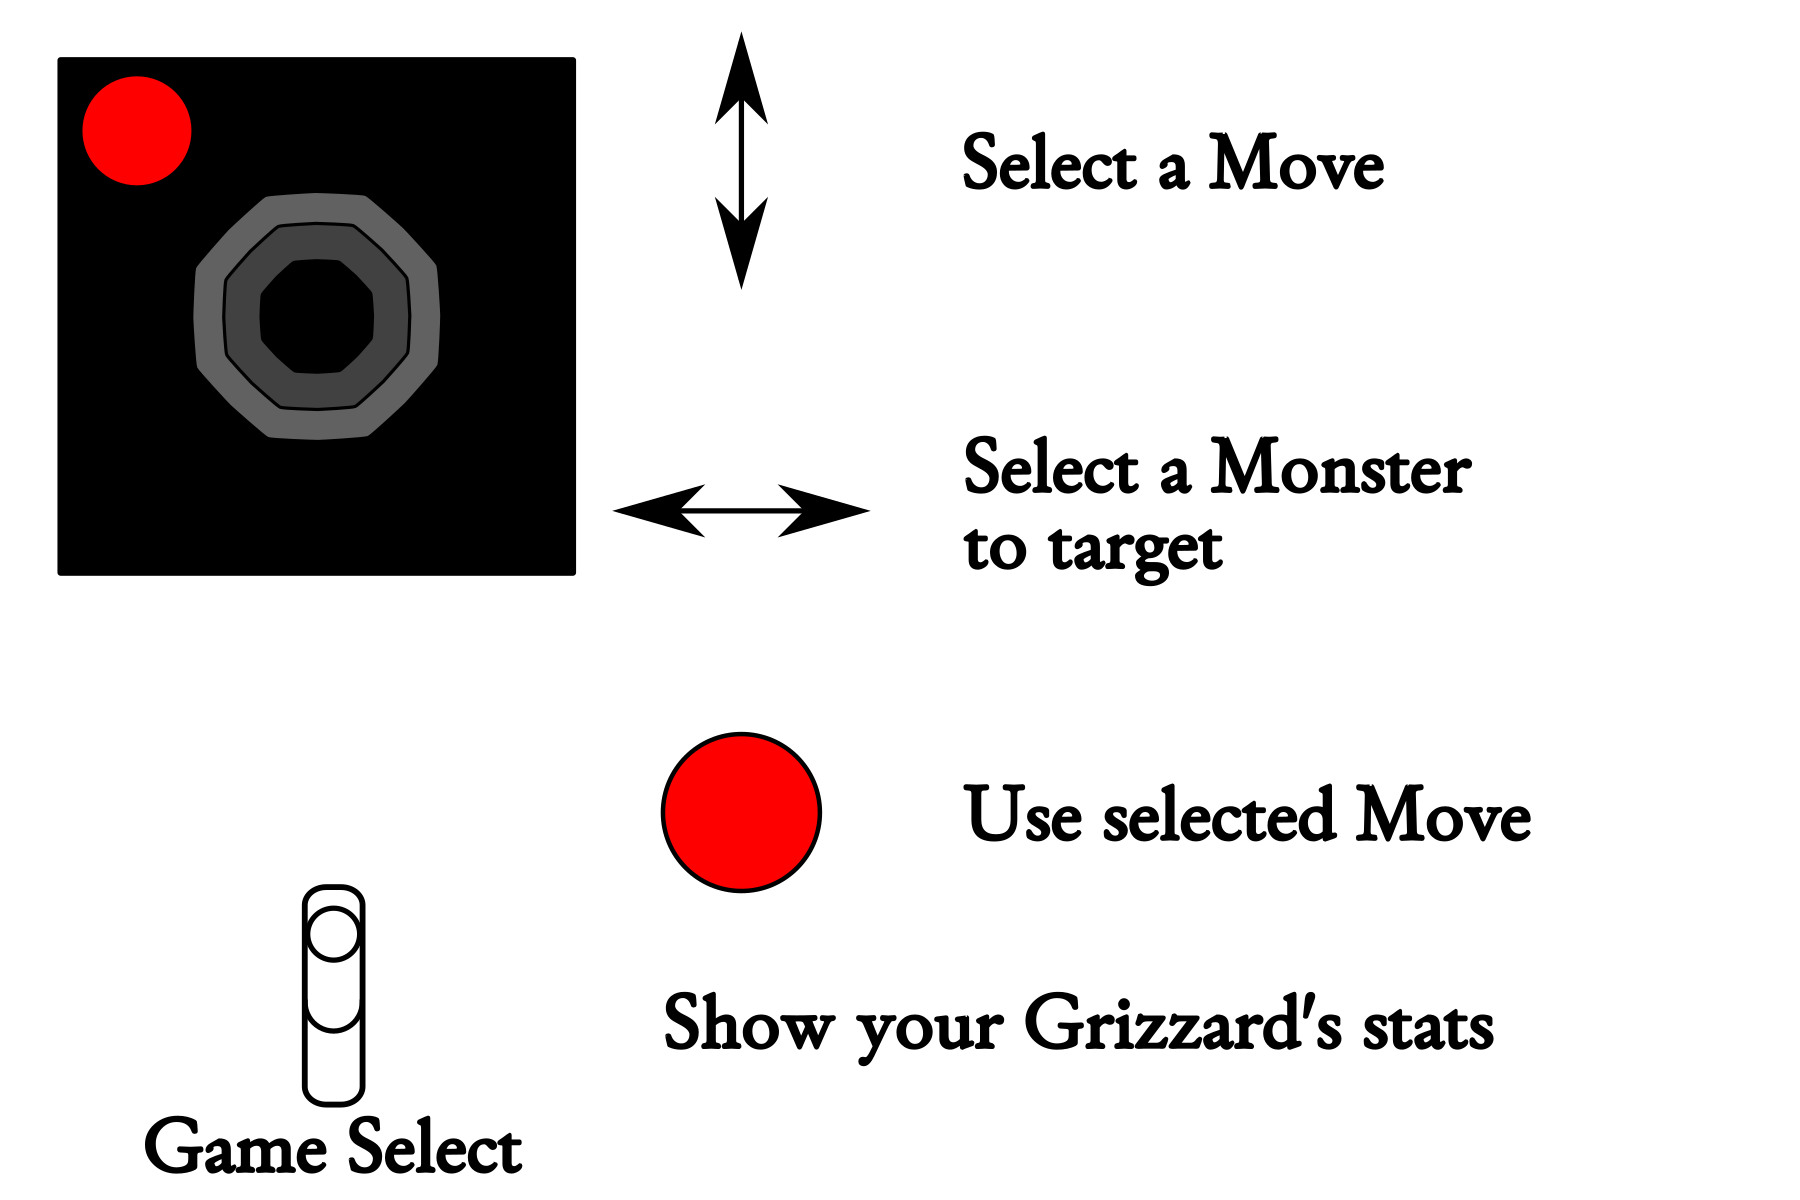
\includegraphics[width=2\columnwidth]{../Manual/CombatControls.png}
\end{figure*}

When you  encounter monsters, you'll  see the Combat display.  When it's
your turn, the bottom part of the screen (showing your Grizzard) will be
\ifdefined\TVSECAM magenta\else  indigo\fi{}. The long bar  beneath your
Grizzard shows its hit points.

\begin{center}
  \includegraphics[width=\columnwidth]{../Manual/GrizzardCombat\TV.png}
\end{center}

When  it's the  monsters'  turn, the  top  part of  the  screen will  be
\ifdefined\TVSECAM white. \else red. \fi

\begin{center}
  \includegraphics[width=\columnwidth]{../Manual/MonsterCombat\TV.png}
\end{center}

Monsters often  travel in groups, so  you may see more  than one monster
facing you.

You can choose  from the moves that your Grizzard  knows how to perform.
Press the joystick  forward and back to select a  move. If your Grizzard
knows how to perform it, it will  appear in light blue. If your Grizzard
does not yet know how, it will appear in black.

Most Moves will target one monster.  Press left or right on the joystick
to select a target. Some Moves instead affect yourself.

When   you   have   chosen   a   move  (and   a   target),   press   the
\textbf{Fire} button.

To view the statistics of your Grizzard, press \textbf{Game Select}.

\subsection{Performing a Move}

\begin{figure*}[b]
  \begin{center}
    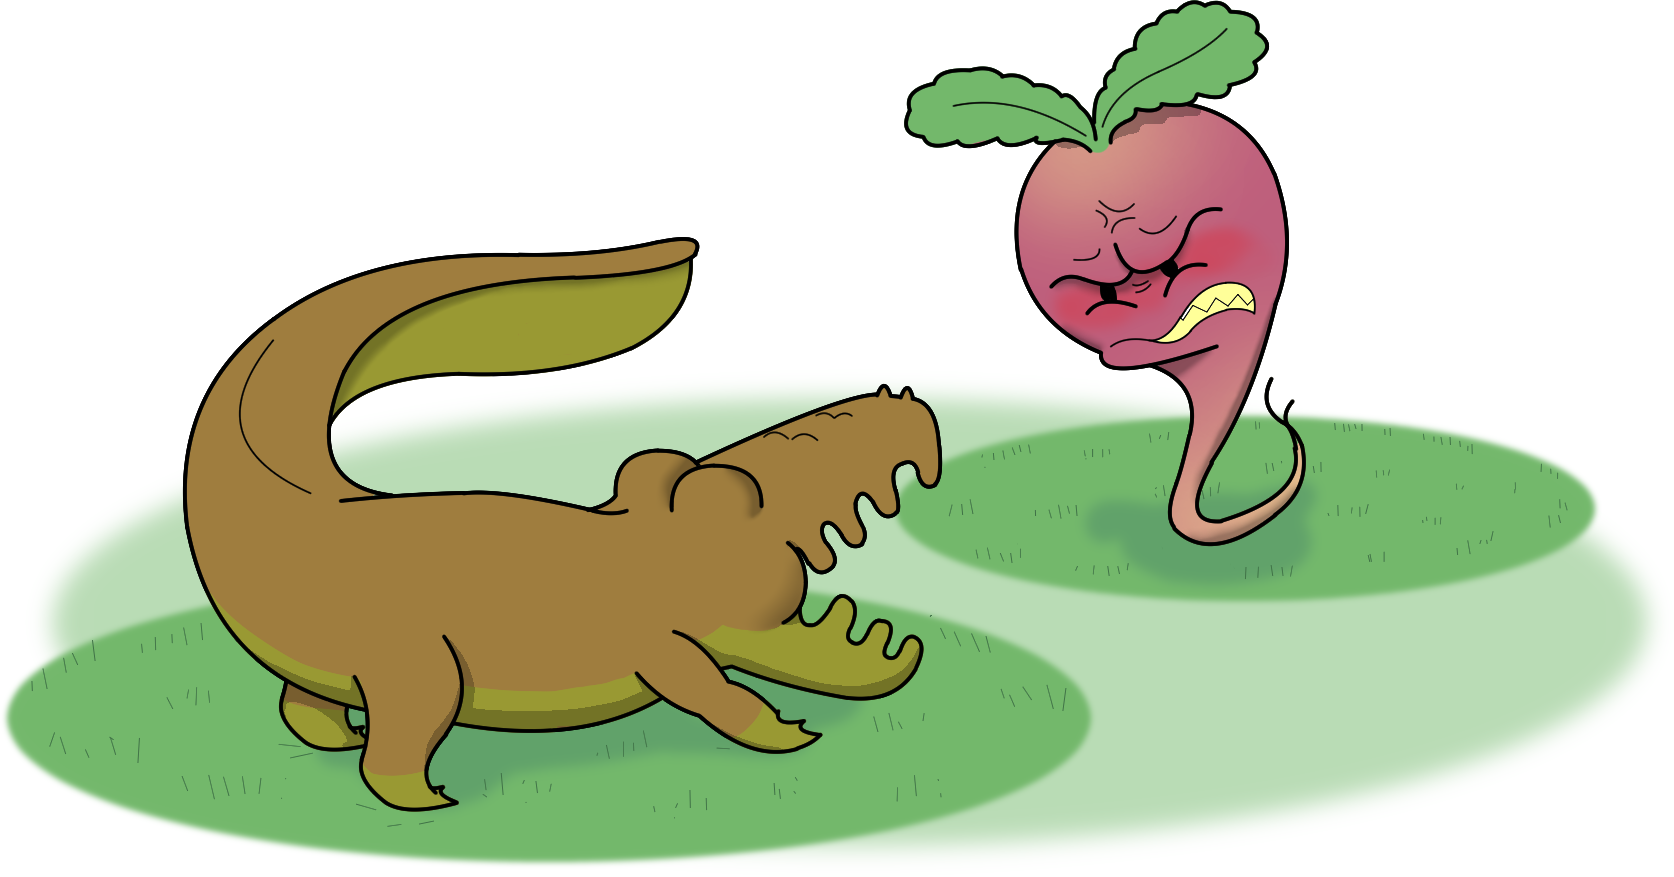
\includegraphics[width=2\columnwidth,height=\columnwidth]{../Manual/GrizzardCombat.png}
  \end{center}
\end{figure*}

After a move has been performed,  the creature targeted by that move may
be injured  (lose hit points)  and/or have a  Status Effect\footnote{See
  page~\pageref{sec:StatusEffects} to learn  about Status Effects} added
to  it. Status  Effects  are temporary  and last  only  the duration  of
one battle.

It's possible for a move to miss its target. If that happens, you'll see
\texttt{MISSED} appear  briefly. It's also  possible to have  a critical
success  ---  that  move  will  do double  the  usual  damage,  and  see
\texttt{CRIT!} appear on the screen.

If your Grizzard companion loses hit points, the bar below your Grizzard
will reduce in  length. If your Grizzard is defeated,  the monsters will
surely eat you! Your adventure will end there. \ifdefined\NOSAVE You can
resume your game from the Begin/Resume  screen, or start over. \else You
can continue from  the last Grizzard Depot you visited  by selecting the
same game slot on the Select Slot screen. \fi

If you  defeat all of  the monsters, victory  is yours! Your  score will
increase, and you'll  return to the World Map screen.  You may also find
a potion was  left behind by the monsters. \ifdefined\DEMO  There are no
potions in the demo. \fi

You  may choose  to run  away from  a fight,  but the  monsters will  be
immediately healed and may still come after you.

\subsection{Grizzard Learning}

Your  Grizzard companion  may  learn from  opposing  Monsters. This  can
result in your Grizzard increasing  its Attack or Defend rating, maximum
hit points, or learning a new Move. Your Grizzard can only learn certain
Moves. Moves that  your Grizzard might be able to  perform, but does not
yet  know, will  appear in  black. Sometimes,  seeing a  monster perform
a Move  will teach it to  your Grizzard. Other times,  your Grizzard may
work it out on their own.

\section{Statistics}

\begin{center}
  \includegraphics[width=\columnwidth]{../Manual/StatsScreenshot\TV.png}
\end{center}

You can  press the  \textbf{Game Select} switch  while viewing  the Map,
Combat  screen,  or  at  a   Grizzard  Depot  to  view  your  Grizzard's
statistics.   Press  the   \textbf{Fire}   button  to   return  to   the
previous screen.

At  the top  of the  Statistics screen,  you'll see  a portrait  of your
Grizzard companion,  their name, and  their unique number. There  are 30
Grizzards to catch. Can you catch them all?

\begin{description}
  
\item[\texttt{ATK.}] is the Grizzard's  \emph{attack} rating. This is the
  likelihood  that your  Grizzard  will  hit and  cause  damage when  it
  attacks a monster. Some Moves cause more damage than others.
  
\item[\texttt{DEF.}] is the Grizzard's  \emph{defend} rating. This is how
  likely your Grizzard is to avoid being hurt by a monster's Move.

\item[\texttt{HP}]  is  the  Grizzard's  \emph{hit  points}  or  health.
  When  monsters hit  your Grizzard,  this  value will  decrease. If  it
  reaches zero, your game is over.

\item[\texttt{MAX}]  is   the  Grizzard's  \emph{maximum   hit  points}.
  Your Grizzard can gain more hit points up to this amount.
  
\end{description}

Each of  these statistics can  be raised up to  a maximum of  99 points.
The Attack  rating, Defend  rating, or  Maximum Hit  Points may  go up
a bit after each monster that you defeat. The more skilled your Grizzard
becomes, the less often its levels will go up.

If you are currently in a  combat encounter, there may be Status Effects
that could change the effectiveness  of your Moves. These are \emph{not}
displayed on the statistics screen.

\section{Status Effects}\label{sec:StatusEffects}

A move can affect its target with Status Effects. There are six possible
Status Effects:

\begin{description}
\item[\texttt{SLEEP}] A  creature can not  move on their turn.  There is
  a 50\% chance of waking up.
\item[\texttt{ATK UP} / \texttt{ATK DN}] Raises or lowers the creature's
  effective Attack rating.
\item[\texttt{DEF UP} / \texttt{DEF DN}] Raises or lowers the creature's
  effective Defend rating.
\item[\texttt{MUDDLE}]  A  creature will  choose  its  moves at  random.
  There is a 50\% chance of clearing its mind.
\end{description}

These status effects last only the duration of one battle.

Also, these status effects cannot be  doubled up. For example: Once your
attack has been raised, it cannot be raised further.

\section{Scoring}

When you  defeat a monster, you'll  earn points. The number  of points
you earn  will increase as you  defeat more difficult monsters.  You can
also earn points for other some other actions you take in the game.

The score earned can be increased by:

\begin{itemize}
\item \ldots{}playing  in Expert  mode (by  setting the  Left Difficulty
  Switch to the ``A'' position)
\item \ldots{}defeating the larger version of a monster
\item  \ldots{}playing the  game  in  New Game  Plus  mode after  having
  defeated the final boss.
\end{itemize}

The score for  defeating a monster will be increased  to $2\times$ for any
one of these  factors, to $3\times$ for  any two of these  factors, and to
$4\times$ if all three are true.

\section{Winning the Game}

You can  win the  game by  discovering what dark  forces are  behind the
onslaught of so many monsters, and defeating them.

\subsection*{New Game Plus}\label{sec:NewGamePlus}

Once  you've won  the game,  you can  keep playing!  On the  screen that
appears when you win, press \textbf{Game  Reset} on your console to save
your winning score and create a ``new game, plus.''

On your second time through, you'll  have both of the starting Grizzards
that you  had not  chosen the first  time, as well  as all  your trained
Grizzards to choose from. Monsters will become more difficult — but also
yield more points when defeated.

\section{Game Over}

If  you fail  in  your mission,  your  game is  over.  However, you  can
continue, and it'll be just as if you'd never failed in the first place.
You'll start over from \ifdefined\NOSAVE the beginning of the game, with
your  current progress.  \else  the  last Grizzard  Depot  that you  had
visited. \fi

\begin{center}
  \includegraphics[width=\columnwidth]{../Manual/GameOver\TV.png}
\end{center}

\section{Starting Over}\label{Starting Your Adventure Over}

\ifdefined\NOSAVE

When  you  start  the  game,  you can  \texttt{BEGIN}  a  new  game,  or
\texttt{RESUME}  your existing  game.  If  you begin  a  new game,  your
previous progress will be erased.

\else

If you want to erase your progress and start again, you must:

\begin{itemize}
\item Go  to the Select Slot  screen, and press \textbf{Game  Select} or
  move  the joystick  left and  right until  you see  the slot  you want
  to erase.
\item Set both  of the Difficulty Switches on your  console to the ``A''
  (Advanced or Expert) position.
\item With your  joystick controller, pull back  and \emph{while holding
    the joystick back} press and hold the \textbf{Fire} button.
\item If you're \emph{sure} you want to erase your game's progress, then
  \emph{without}  letting  go  of  the \textbf{Fire}  button,  move  the
  joystick  forward. \ifdefined\DEMO  Your  game record  will be  erased
  \emph{immediately}. \fi
\end{itemize}

\begin{center}
  \includegraphics[width=\columnwidth]{../Manual/EraseSlot\TV.png}
\end{center}

\ifdefined\DEMO

\emph{Once your game record has been  erased, you can not recover it, so
  think carefully before you erase it.}

\else

Make sure  you want to  erase your game.  Press the joystick  forward or
back to make your choice, and press the \textbf{Fire} button.

\begin{center}
  \includegraphics[width=\columnwidth]{../Manual/ConfirmErase\TV.png}
\end{center}

\fi

The Left  Difficulty Switch is also  used to increase the  difficulty of
the game. After  erasing your progress, you may want  to return the Left
Difficulty Switch to your desired position.


\ifdefined\TVSECAM

The  Right   Difficulty  Switch  is   also  used  to  pause   the  game.
After erasing your  progress, return the Right Difficulty  Switch to the
``B'' position.

\fi

\subsection{Protecting Your Game Record}

If  either of  your Difficulty  Switches is  in the  ``B'' (Beginner  or
Novice) position, you can't erase a game slot.

\ifdefined\DEMO\else

\subsection{Recovering an Erased Game}

If you have just erased a game's  progress, and no one has started a new
game using the same slot yet, you may be able to un-erase it.

To recover  an erased game,  follow the same steps  as if you  wanted to
erase  a game.  Press  left and  right  on the  joystick  to select  the
now-empty  slot  (the  screen  will say  ``\texttt{BEGIN}'').  Set  both
Difficulty Switches  to the  ``A'' (Advanced  or Export)  position, pull
back  on  the joystick,  and  \emph{while  holding  it back},  hold  the
\textbf{Fire} button.

If your  game's progress can be  recovered, you'll see that  the slot is
\texttt{ERASED} and you should also see your name appear. To recover the
game's progress, press forward on the joystick. The game will immediately
become available to resume.

Note that it  is \emph{not possible} to recover a  saved game's progress
once  a new  game has  been  started in  the  same memory  slot. If  you
accidentally start  a new game,  but have  not confirmed your  name yet,
\emph{turn off the power briefly}, then try the recovery steps above.

\fi

\fi % not-nosave

\columnbreak
\chapter{Grizzards and Moves}
\label{ch:Grizzards}

There are  30 Grizzards in  the game world,  each with their  own unique
starting attributes and sets of Moves.

\ifdefined\NOSAVE

In  this  demo,  you  can  play  with  only  one  Grizzard  at  a  time.
Other   Grizzards  are   available   with  a   memory   device  or   the
retail cartridge.

\fi

Each Grizzard is able  to learn up to 8 different  moves, in addition to
the move \texttt{RUN AWAY}. It's up  to you to discover which Moves each
Grizzard is able to learn.

\ifdefined\DEMO\else

\section{Dirtex}

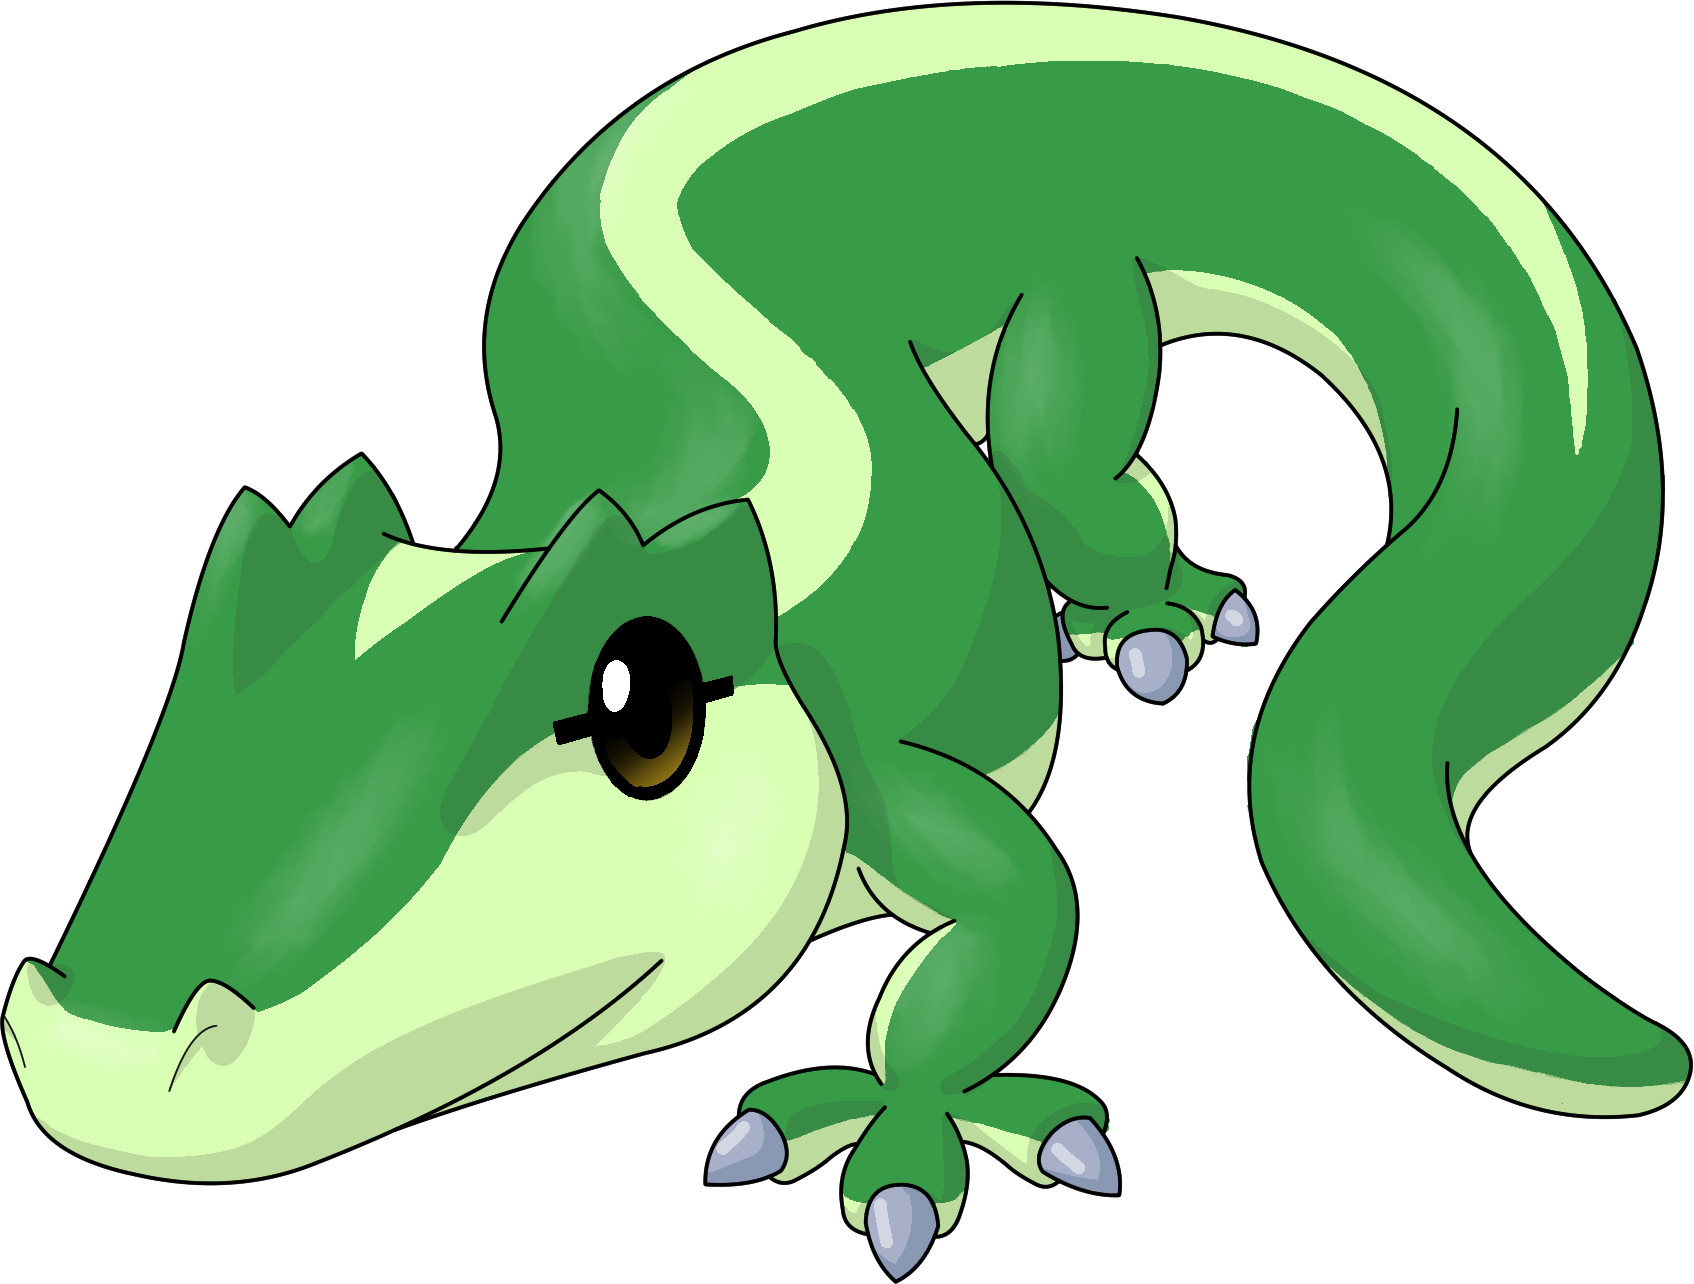
\includegraphics[width=\columnwidth]{../Manual/Dirtex.png}

The green  Dirtex Grizzard (Num. 01)  lives in the desert.  It can learn
these Moves:

\begin{itemize}
\item \texttt{KICK DIRT} --- kick dirt at the enemy, causing some damage
  to them.
\item \texttt{BURY DEEP} --- try to bury the enemy, which may cause them
  to fall asleep.
\item  \texttt{DIRTY FOOT}  --- causes  some  damage and  may lower  the
  enemy's defend value.
\item \texttt{LOAMY FEAR} --- may lower the enemy's attack value.
\item \texttt{DUSTY EYES} --- may lower the enemy's defend value.
\end{itemize}

Dirtex may, if it gains enough experience, metamorphose into Lander.

\fi

\section{Aquax}

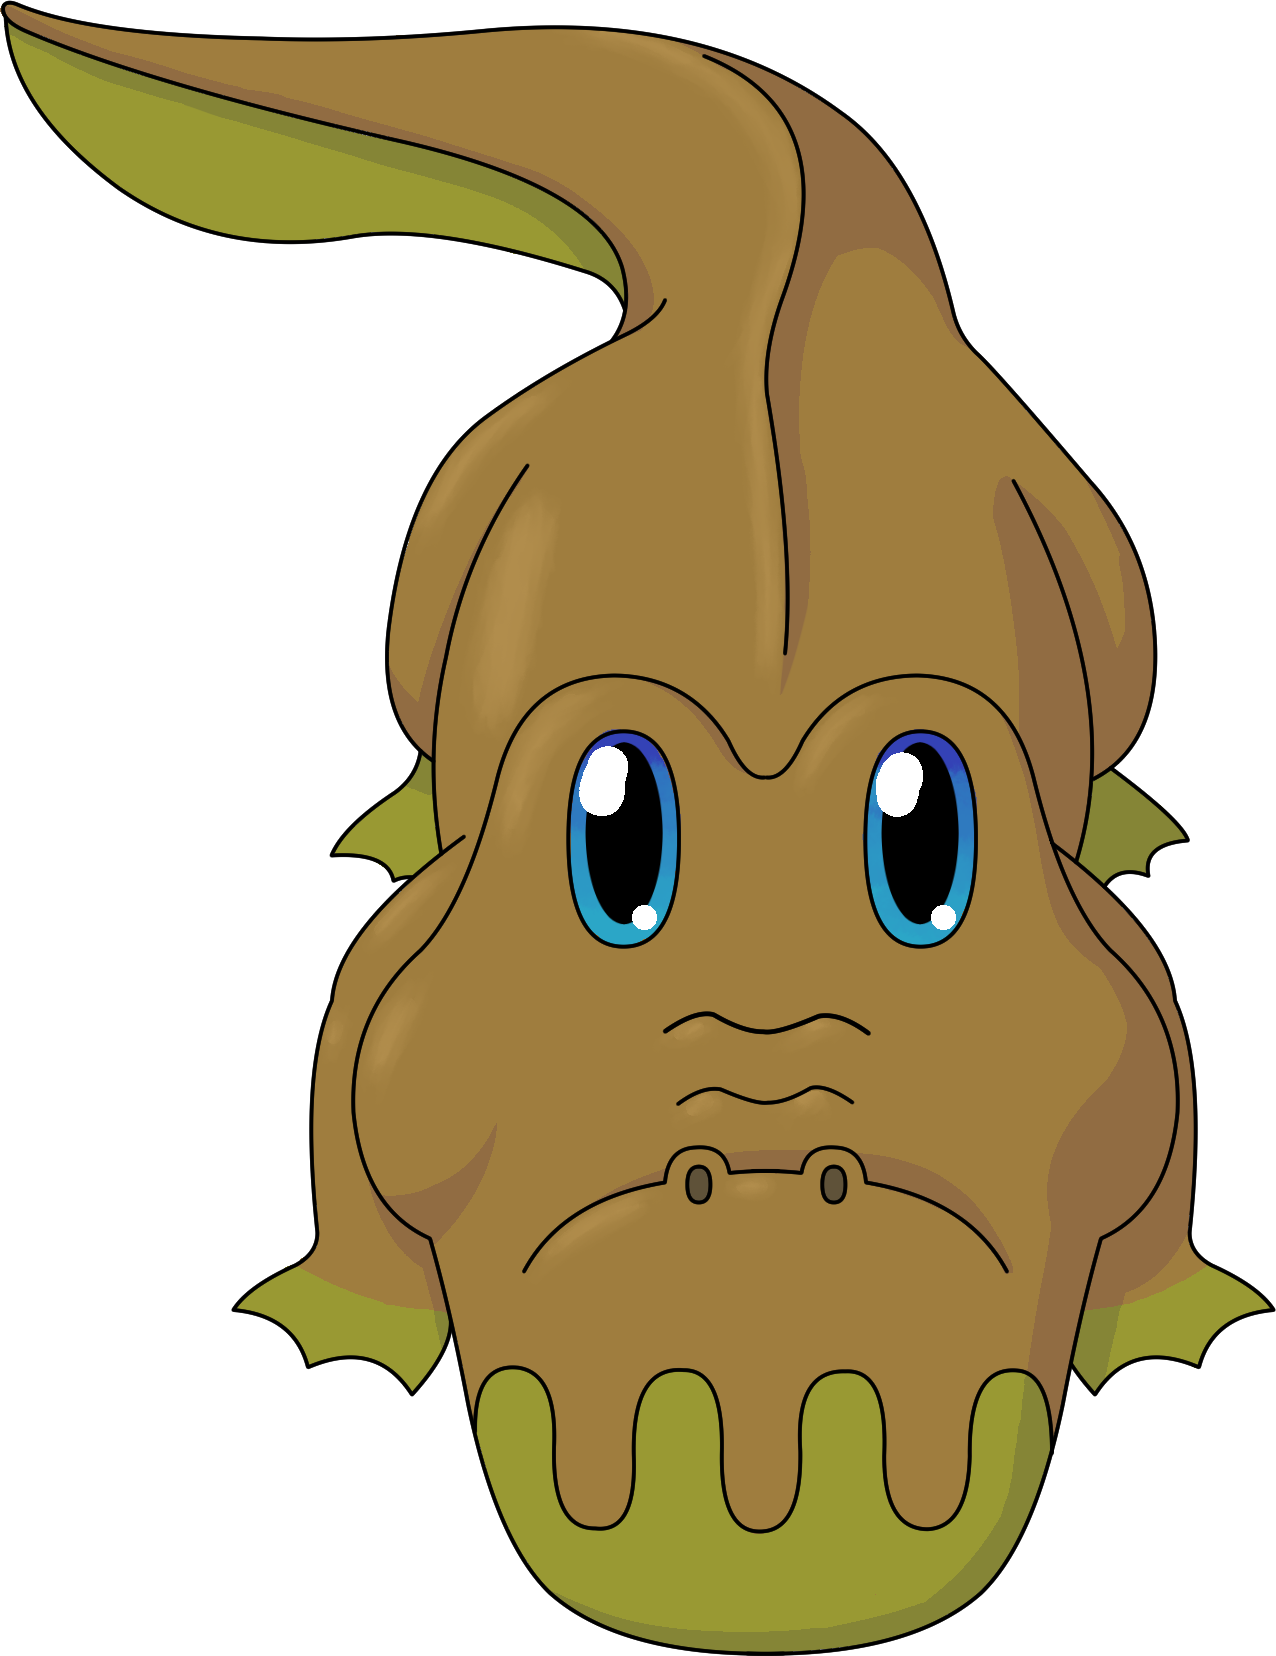
\includegraphics[width=\columnwidth]{../Manual/Aquax.png}

Aquax is  a brown Grizzard  (Num. 02) which lives  in the water.  It can
learn these Moves:

\begin{itemize}
\item  \texttt{SPLISH SPLASH}  --- splash  water at  the enemy,  causing
  some damage. 
\item \texttt{RAISE HOPE} --- may increase its own defend ability.
\item \texttt{SURE SPLASH} --- may increase its own attack ability.
\item \texttt{QUICK FOOT}  --- causes some damage and  may also decrease
  the enemy's defend ability.
\item \texttt{GREAT MOJO}  --- causes some damage and  may also decrease
  the enemy's attack ability.
\end{itemize}

With enough experience, Aquax can metamorphose into Sailor.

\ifdefined\DEMO\else

\section{Airex}

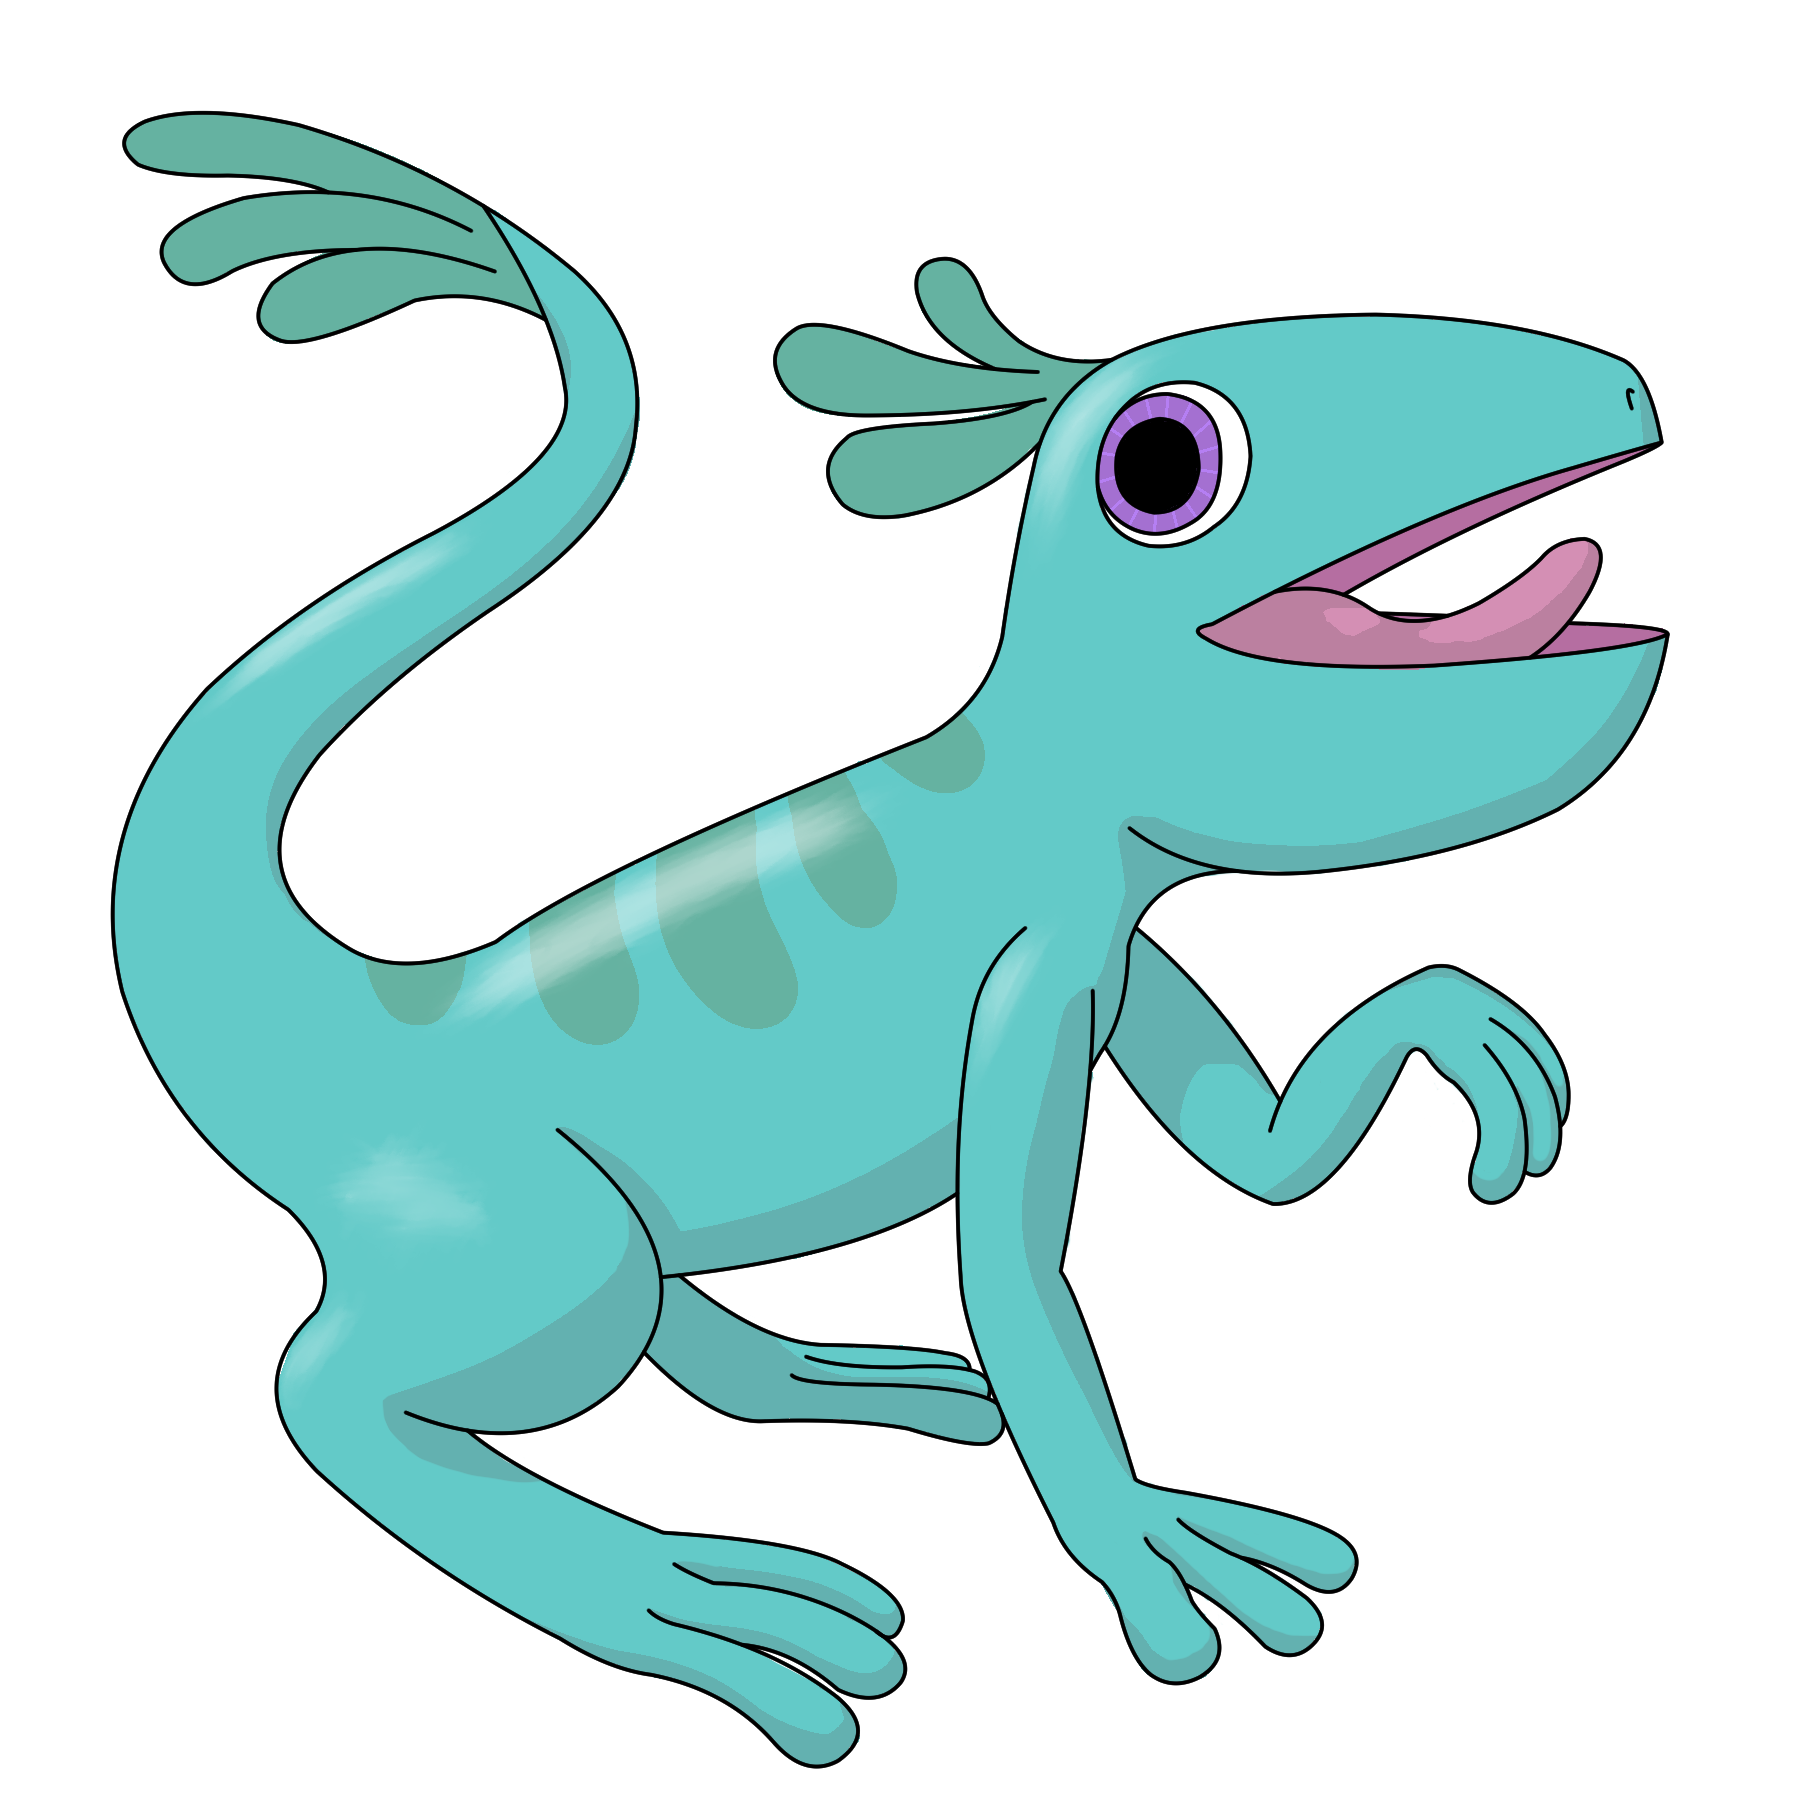
\includegraphics[width=\columnwidth]{../Manual/Airex.png}

Airex is  a teal  Grizzard (Num. 03)  which lives in  the trees.  It can
learn these Moves:

\begin{itemize}
\item \texttt{MILD SHOCK} --- shocks  the enemy with static electricity,
  causing some damage.
\item \texttt{WIND FIGHT} --- causes a bit more damage than \texttt{MILD SHOCK}
\item \texttt{STEAL ATTACK} --- may lower the enemy's attack value.
\item \texttt{STEAL DEFEND} --- may lower the enemy's defend value.
\item \texttt{STEAL TURN} --- may put the enemy to sleep
\end{itemize}

If Airex gains enough experience, it will metamorphose into Flyer.

\fi

\section{Healing}

Most Grizzards can learn healing moves as well. Some examples:

\begin{itemize}
\item \texttt{FIRST  AID} ---  heals a small  amount of  health, raising
  your own hit points.
\item \texttt{SIMPLE CURE} --- heals a bit larger amount of health.
\item \texttt{COMMON CURE} --- heals even more health.
\end{itemize}

You can also heal your Grizzard  by visiting a Grizzard Depot, or giving
them a healing  Potion. To use a potion, press  the \textbf{Fire} button
while on  the map  screen. You  can not  use a  potion during  a battle.
\ifdefined\DEMO There are no potions in this demo. \fi

\section{Run Away}

This Move lets you try to escape from a battle.

Your  Grizzard will  \emph{not}  be  healed if  you  run  away, but  the
monsters that you were facing will be healed immediately.

Certain  monsters  are too  terrifying  to  escape. When  you  encounter
a ``boss'' monster like that, it will  be a duel to the death. Watch out
for their unique shape on the map.

\section{Metamorphosis}

Many Grizzards  can metamorphose into a  new form when they  have gained
a certain amount  of experience by battling monsters.  Each Grizzard has
their  own experience;  they only  gain experience  when they  battle as
your companion.

When  a Grizzard  undergoes  metamorphosis, you'll  see an  announcement
screen  \ifdefined\DEMO  which  looks   as  though  you've  just  caught
a new Grizzard. In the full game, it's more obvious that this is because
of  a  metamorphosis. \else  which  shows  the Grizzard's  previous  and
new forms. \fi

\columnbreak
\chapter{Monsters}

Terrible monsters are  arriving in Syrex, terrorizing the  people. A few
of them are described here.

\vspace{14pt}

\lettrine[image=true,                lines=5,               findent=3pt,
nindent=3pt]{../Manual/Wicked-Slime.png}{Wicked}  Slimes are  weak slime
monsters that  your Grizzard can  kill fairly  easily … but  beware when
they travel in large packs. Like  many creatures, they know some healing
Moves that  might be useful to  learn. Wicked Slimes are  now found near
Treble Village and the Lost Mine.

\vspace{14pt}

\lettrine[image=true,                lines=5,               findent=3pt,
nindent=3pt]{../Manual/Horrid-Slime.png}{Horrid}    Slimes   are    more
dangerous than a  Wicked Slime. A Horrid Slime may  survive your attacks
until you've learned some new moves.

\vspace{14pt}

\lettrine[image=true,                lines=5,               findent=3pt,
nindent=3pt]{../Manual/Vorpal-Bunny.png}{Vorpal} Bunnies  are a powerful
monster that will take a few hits  to kill, but they're the only way for
Aquax to  learn Great Mojo. Beware  their attack Moves, though!  You may
find Vorpal Bunnies near the Spiral Woods.

\vspace{14pt}

\lettrine[image=true,                lines=5,               findent=3pt,
nindent=3pt]{../Manual/R.O.U.S..png}{Rodents} of Unusual Size are one of
the  dangers of  the Fire  Bog (but  I don't  think they  really exist).
They're known to attack pirates and princesses alike.

\vspace{14pt}

\lettrine[image=true,                lines=5,               findent=3pt,
nindent=3pt]{../Manual/Flame-Doggo.png}{Flame  Doggos} are  a danger  of
the Fire  Bogs. These beasts  often roam in packs,  and their fur  is on
fire. Avoid the Fire Bogs until you have begun to train your Grizzard to
have a higher Attack stat.

\vspace{14pt}

\lettrine[image=true,                lines=5,               findent=3pt,
nindent=3pt]{../Manual/Will-O-Wisp.png}{Will-O-Wisps}     are    bright,
floating sparks  that are  known to  travel in  large groups.  Once your
Attack rating is high enough to hit them, they go down quickly, but they
have very strong defenses!

\vspace{14pt}

\lettrine[image=true,                lines=5,               findent=3pt,
nindent=3pt]{../Manual/Lectro-Sheep.png}{Lectro  Sheep}   are  dangerous
sheep that are full of static electricity. They roam the countryside, as
sheep will do.

\vspace{14pt}

\lettrine[image=true,                lines=5,               findent=3pt,
nindent=3pt]{../Manual/Viking-Turtle.png}{Viking Turtles}  are dangerous
waterfront creatures that can be very dangerous to encounter.

\vspace{14pt}

\lettrine[image=true,                lines=5,               findent=3pt,
nindent=3pt]{../Manual/Crazy-Fox.png}{Crazy Foxes} are likely to unleash
a great deal of  pain. It's said that they were  never actually foxes to
begin with, but were created already crazy.

\vspace{14pt}

\lettrine[image=true,                lines=5,               findent=3pt,
nindent=3pt]{../Manual/Water-Kitty.png}{Water  Kitties}  are  a  special
kind of  cat that likes to  swim, and to dish  out punishing water-based
attacks on anyone who comes near them.

\vspace{14pt}

\lettrine[image=true,                lines=5,               findent=3pt,
nindent=3pt]{../Manual/Creepy-Spider.png}{Creepy   Spiders}   are   much
bigger than  the sort  where you  come from. Watch  out for  those giant
mandibles, they hurt!

\vspace{14pt}

\lettrine[image=true,                lines=5,               findent=3pt,
nindent=3pt]{../Manual/Metal-Mouse.png}{Metal   Mice}    are   extremely
durable, so it  can take a while  to chip away at their  hit points, but
the rewards in points earned may well be worth it.

\vspace{14pt}

\lettrine[image=true,                lines=5,               findent=3pt,
nindent=3pt]{../Manual/Fire-Panda.png}{Fire Pandas}  are a bit  like red
pandas, or firefoxes, and quite a  bit more dangerous. Unlike a firefox,
these beasts actually dish out fire-based attacks on their victims.

\section*{and many more...}

There  are many  other monsters  roaming the  countryside across  Syrex.
You'll have to discover the others on your own. Here's a hint: There are
more than 40 types of monsters that  you can face, and most of them also
can be found in more powerful giant forms as well.

}

\ifdefined\ATARIAGESAVE\else

\columnbreak
\chapter{Troubleshooting}

\ifdefined\DEMO

\section*{Screen ``Jitters,'' freezes,  \ifdefined\TVPAL appears in black
  \& white,\fi or flashes blue}

These may  be signs that  a screen  (or the transition  between screens)
does not have the correct ``scan line'' count. This is a technical error
by the game's  developer (that's me!) and must be  corrected in the next
build of the game.

If you see these  effects (or if you are running in  an emulator, if you
notice that the  scan line count is not \ifdefined\TVNTSC  262 \else 312
\fi      at     all      times)      please      report     them      to
\hred{mailto:support@star-hope.org}{support@star-hope.org} so  that they
can be corrected before the game is finished.

\fi

\section*{Sad Face Screen}

If you  see the Sad  Face screen,  the game is  trying to tell  you that
there is a problem.

From here, you can press the \textbf{Game Reset} switch to return to the
Title Screen.

\ifdefined\ATARIAGESAVE\else\ifdefined\NOSAVE\else

\subsection{Red Sad Face Screen: Memory Device Needed}

\includegraphics[width=\columnwidth]{../Manual/RedSadFace\TV.png}

Your  memory device  was not  found.  Connect an  AtariVox, SaveKey,  or
MemCard to the  right controller port. You should also  plug in speakers
or headphones to your AtariVox to hear game voices.

\fi\fi

\subsection{White Sad Face Screen}

\includegraphics[width=\columnwidth]{../Manual/WhiteSadFace\TV.png}

The game  has encountered an  error and cannot continue.  Please contact
\href{mailto:support@star-hope.org}{support@star-hope.org}           for
additional assistance. Send the code  number that appears on this screen
with your email.

\ifdefined\ATARIAGESAVE\else

\section*{Pause button must be held down (7800)}

This  is believed  to  be  a side  effect  of  certain multi-carts,  eg.
PlusCart.  Note that  you can  press \textbf{Game  Select} to  view your
Grizzard's statistics and effectively pause the game as well.

\fi

\ifdefined\NOSAVE\else\ifdefined\ATARIAGESAVE\else

\section*{TV goes blank when entering Grizzard Depot}

Make  sure your  memory device  is  securely connected.  If your  memory
device is not connected when the game  tries to save, you may see the TV
picture remain blank while the game tries to record your progress.

\fi

\section*{No voices}

On the title  screen, you'll hear the AtariVox announce  the name of the
game. If  you don't, make  sure that the  AtariVox is connected  and the
speakers (or headphones) are connected, powered on, and turned up.

Naturally,  there are  no  voices  when playing  \ifdefined\ATARIAGESAVE
without an AtariVox device. \else with a MemCard or SaveKey device. \fi

\fi

\ifdefined\NOSAVE

\columnbreak
\chapter{No-Save Version}

This special  No-Save demo does not  allow you to save  your progress or
change Grizzards,  but it can be  used without a memory  device (such as
SaveKey, MemCard, or AtariVox). When you turn off power to your console,
all progress is erased.

\fi

\fi % not AtariAge release

\pagebreak
\chapter{Credits}

{\small

  The \textit{Grizzards}  videogame software, including  its audiovisual
  components  and this  manual,  are  copyright \copyright{}  2021-2022,
  Bruce-Robert  Pocock.  All  Rights  are  Reserved  except  as  granted
  under license.

\begin{itemize}
\item Bruce-Robert Pocock --- Programming, Manual text, Graphics,
  Sound effects
\item Zephyr Salz --- Graphics and Printed Artwork; Music
\end{itemize}

\bigskip

Includes VCS  header file by  Matthew Dillon, Olaf  ``Rhialto'' Seibert,
Andrew  Davie, and  Peter H.  Froehlich. Binary  to decimal  translation
based upon  code by  Andrew Jacobs,  based upon  code by  Garth Wilsone.
``Six  Digit Score''  48 pixel  wide  display routines  as explained  on
Stella list  by Erik  Mooney and  Bradford W.  Mott. SaveKey  EEPROM and
AtariVox  speech  synthesis driver  based  upon  code by  Alex  Herbert.
Random  number  generator  by  AtariAge  forum  user  \texttt{Supercat}.
Some  math  functions  by AtariAge  forum  user  \texttt{Omega\-matrix}.
Some  math functions  taken  from December  1984 \textit{Apple  Assembly
  Line}.  ``Have  You   Played  Atari  Today''  jingle   by  Atari  Inc.
transcribed by AtariAge Forum user \texttt{tigger\-the\-hun}. Atari 7800
console detection  logic by Fred  Quimby courtesy of Darrell  Spice, Jr.
AtariVox and SaveKey illustrations in  this manual are from the AtariAge
store.  \ifdefined\ATARIAGESAVE  The AtariAge  logo  and  logotype are  the
property of AtariAge. \fi

Special ``save to cartridge'' circuitry designed by Fred Quimby.

Thanks to Albert Yarusso for publication support.

Special thanks  to everyone in  the Stella and AtariAge  communities for
making this game possible.

\subsection{Testers}

Philip Clark,
James Earl O'Brien,
Darcy Troy Paulin,
\texttt{Mika},
\texttt{vitoco},
David Bowen,
and miscellaneous users from the AtariAge forum.

An early  (alpha) version of the  game's demo was featured  on Zero Page
Homebrew on Twitch on Friday, 6 August, 2021.

\href{https://twitch.tv/zeropagehomebrew}{https://twitch.tv/\-zero\-page\-homebrew}

\href{https://youtu.be/yCFDxUqdP-k?t=4200}{https://youtu.be/\-yCFDxUqdP-k?t=4200}

}

\vfill

\clearpage
\addcontentsline{toc}{chapter}{Map of Syrex}
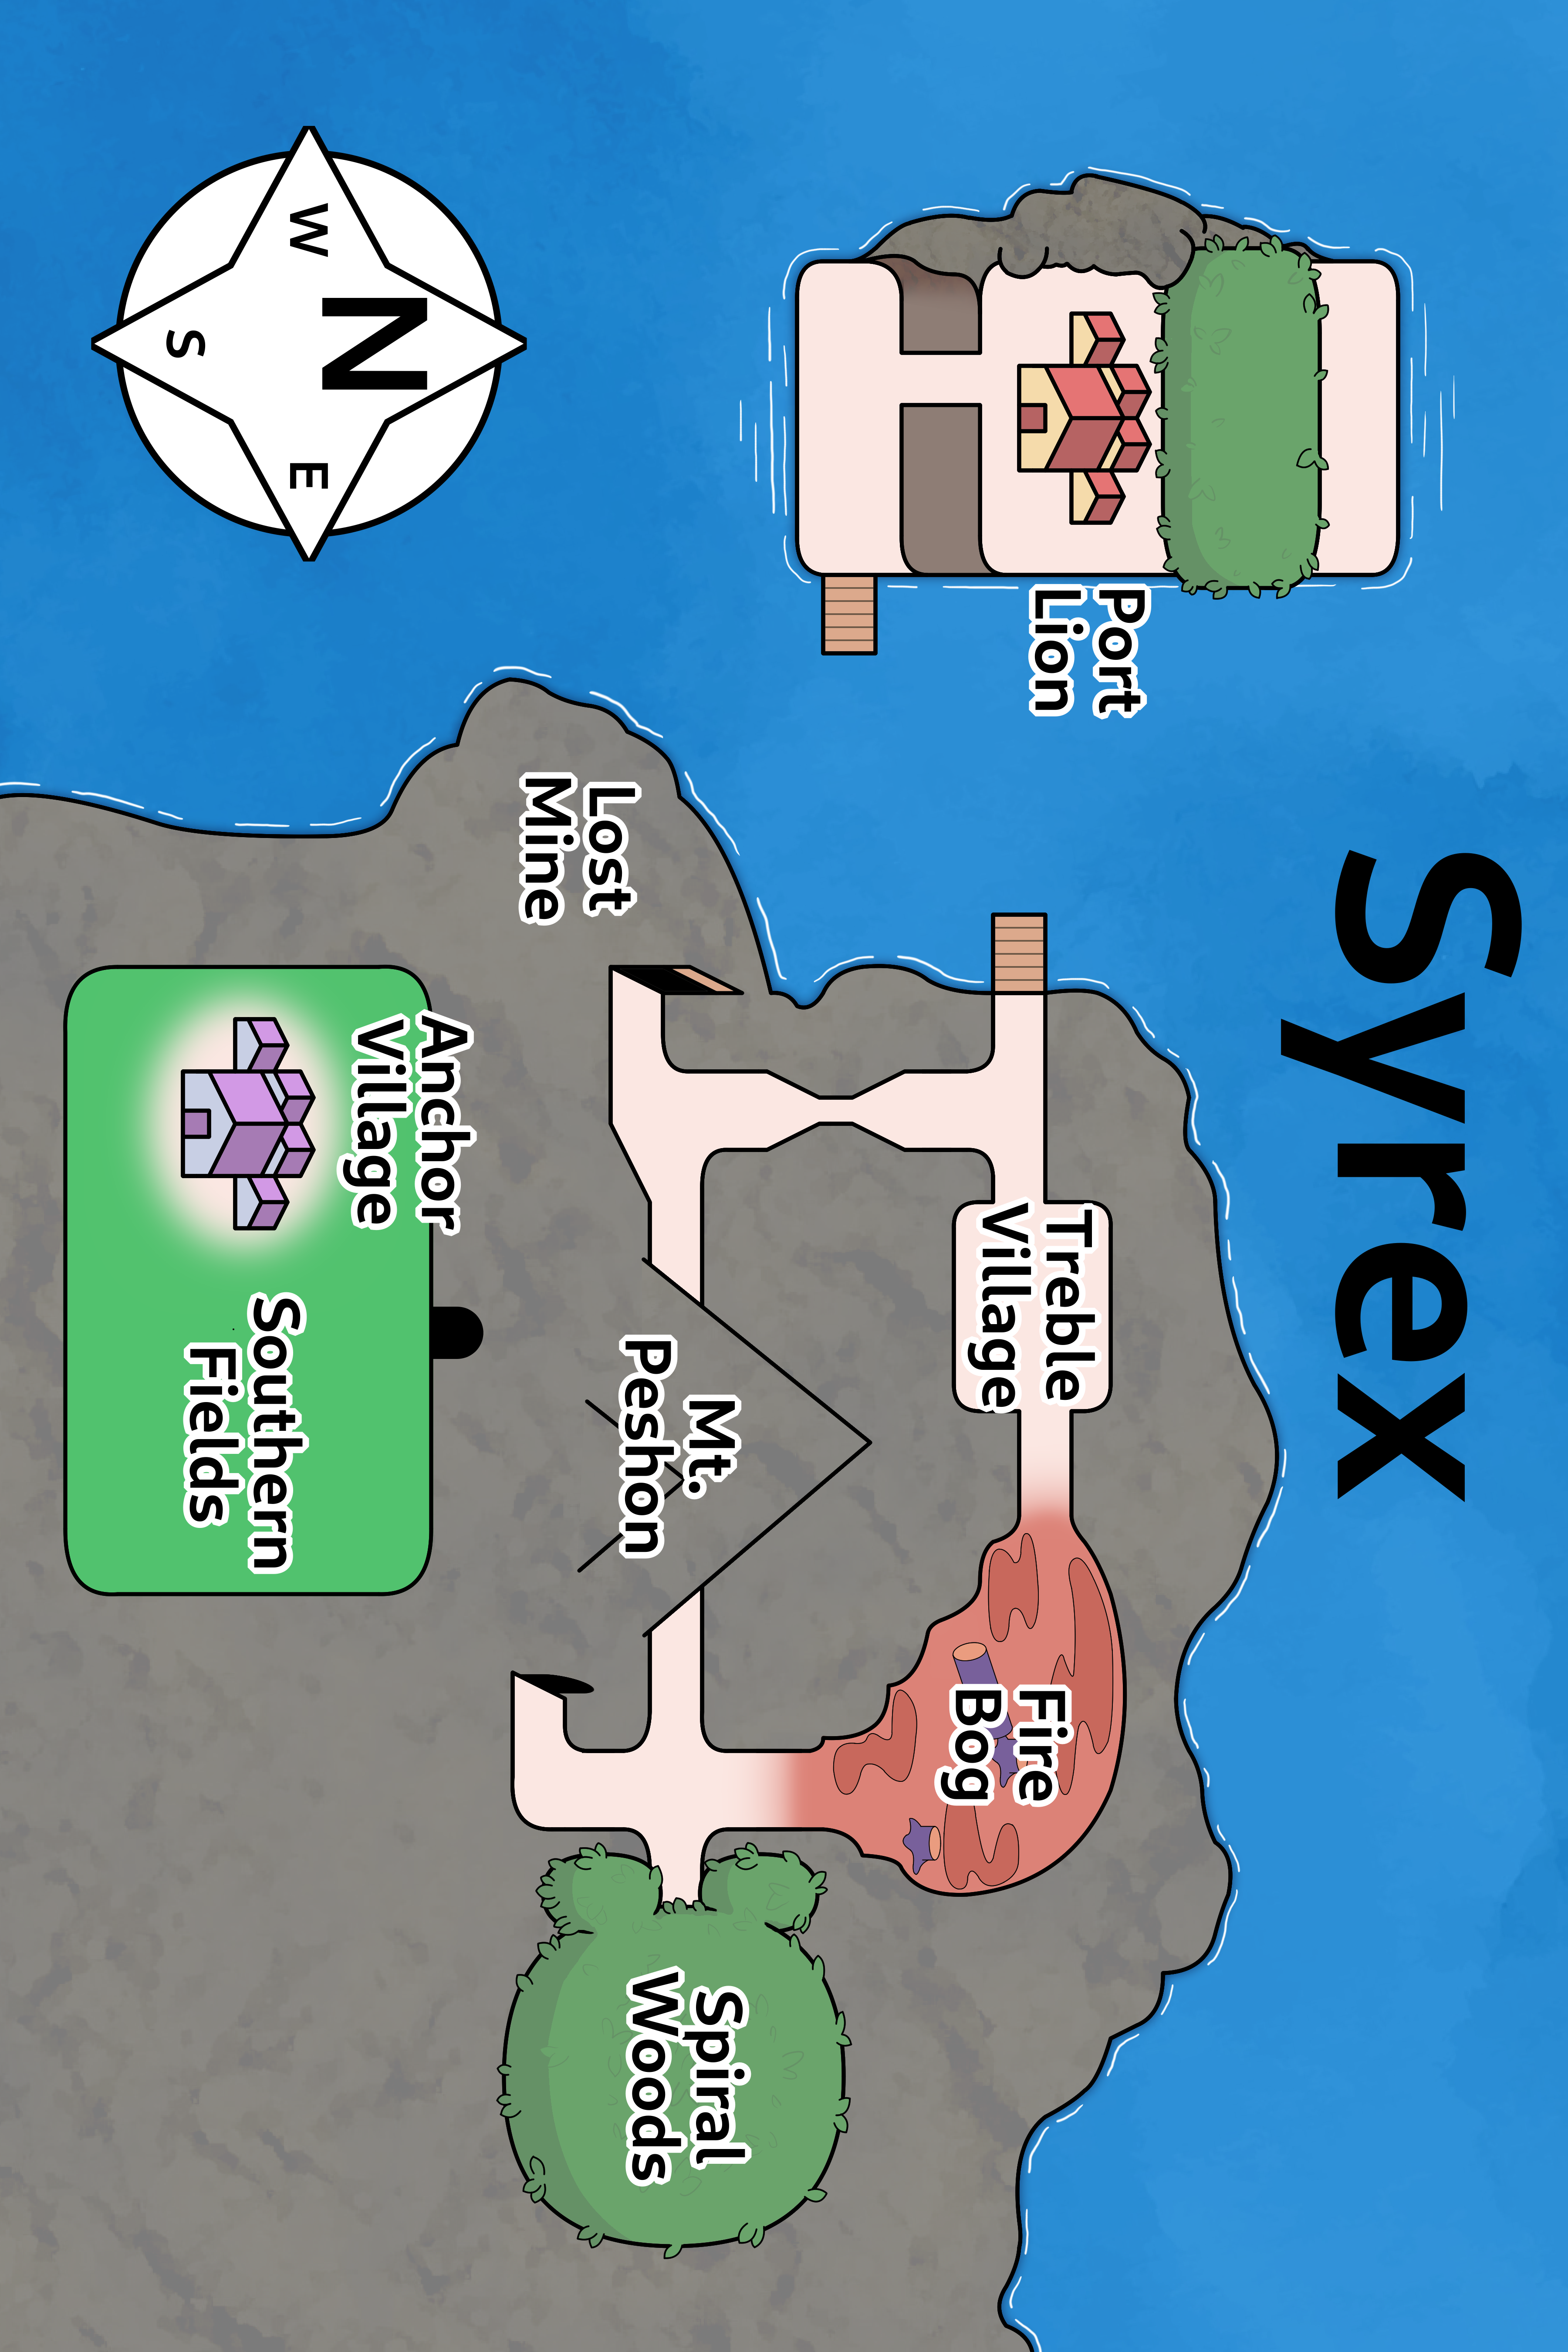
\includepdf[height=9in,width=6in,fitpaper=true]{../Manual/SyrexMap.png}

\end{document}
